\documentclass{scrbook}
\KOMAoptions{
	DIV=12,
	fontsize=12pt,
	paper=letter,
	twoside=false,
	parskip=half-,
}
\usepackage[onehalfspacing, nodisplayskipstretch]{setspace}
\usepackage{amsmath, amssymb, amsfonts}
\usepackage{enumitem}
\setlist[enumerate]{label={(\alph*)}}

\usepackage{tikz}
\usetikzlibrary{arrows, positioning}
\usepackage{subcaption}

\usepackage{xcolor}
\usepackage[
    colorlinks=true,
    linkcolor=blue!60!black,      % For internal links
    citecolor=green!70!black,     % For citation links
    urlcolor=orange!70!black,      % For URLs
    filecolor=cyan!60!black        % For file links
]{hyperref}

\usepackage[canadian]{babel}
\usepackage{csquotes}
\usepackage[showseconds=false, showzone=false]{datetime2}
\DTMsettimestyle{en-CA}

\usepackage{amsthm}
\newtheorem{theorem}{Theorem}
\newtheorem{lemma}[theorem]{Lemma}
\newtheorem{fact}[theorem]{Fact}
\newtheorem{proposition}[theorem]{Proposition}
\newtheorem{corollary}[theorem]{Corollary}
\theoremstyle{definition}
\newtheorem{problem}{Problem}
\newtheorem{question}{Question}
\newtheorem{definition}[theorem]{Definition}
\newtheorem{example}[theorem]{Example}
\newtheorem{remark}[theorem]{Remark}

\newcommand{\vocab}[1]{\textbf{#1}}

\usepackage[mathscr]{eucal}     % For \EuScript
\usepackage{mathtools}
\renewcommand{\geq}{\geqslant}
\renewcommand{\ge}{\geqslant}
\renewcommand{\leq}{\leqslant}
\renewcommand{\le}{\leqslant}
\usepackage{booktabs}
\usepackage{ytableau}
\ytableausetup{centertableaux, smalltableaux}

% Set of Partitions
\DeclareMathOperator\Par{\mathsf{Par}}

% Ring of symmetric functions
\DeclareMathOperator\Sym{\mathsf{\Lambda}}

% Symmetric group
\newcommand{\sym}[1]{\mathscr{S}_{#1}}

% Cycle type
\DeclareMathOperator\cyc{\mathsf{cyc}}

% Inversion number
\DeclareMathOperator\inv{\mathsf{inv}}

% Sign of a permutation
\DeclareMathOperator\sign{\mathsf{sign}}

% Grassmannian
\DeclareMathOperator\Grassmanian{\mathsf{Gr}}

% General Linear group
\makeatletter
\newcommand{\GL}[2][]{%
  \mathsf{GL}%
  \if\relax\detokenize{#1}\relax
    % No optional argument
    (#2)%
  \else
    % Optional argument provided
    _{#1}(#2)%
  \fi
}
\makeatother

% Special Linear group
\makeatletter
\newcommand{\SL}[2][]{%
  \mathsf{SL}%
  \if\relax\detokenize{#1}\relax
    % No optional argument
    (#2)%
  \else
    % Optional argument provided
    _{#1}(#2)%
  \fi
}
\makeatother

% Identity operator
\DeclareMathOperator\id{\mathsf{id}}

% Automorphism group
\DeclareMathOperator\Aut{\mathsf{Aut}}

% Matrix space
\DeclareMathOperator\Mat{\mathcal{M}}

% Hilbert series
\DeclareMathOperator\Hilb{\mathsf{Hilb}}

% Invariant subspace
\DeclareMathOperator\Inv{\mathsf{Inv}}

% Alternating group
\DeclareMathOperator\Alt{\mathsf{Alt}}

% Alternating polynomial
\DeclareMathOperator\AltPoly{\mathsf{AltPoly}}

% Weight of a tableau
\DeclareMathOperator\wt{\mathsf{wt}}

% Set of semistandard Young tableaux
\DeclareMathOperator\SSYT{\mathsf{SSYT}}

% q-binomial coefficient
\newcommand{\qbinom}[3][q]{\genfrac{[}{]}{0pt}{}{#2}{#3}_{#1}}

% Integers
\newcommand{\integers}{\mathbb{Z}}

% Nonnegative integers
\newcommand{\nonnegatives}{\mathbb{N}}

% Positive integers
\newcommand{\positives}{\integers_{> 0}}

% Rational numbers
\newcommand{\rationals}{\mathbb{Q}}

% Real numbers
\newcommand{\reals}{\mathbb{R}}

% Complex numbers
\newcommand{\complexes}{\mathbb{C}}

% Sorted composition
\newcommand{\sort}[1]{\overleftarrow{#1}}

% Finite field
\newcommand{\finitefield}[1]{\mathbb{F}_{#1}}

% Schur function
\newcommand{\schur}[1]{s_{#1}}

% Bender–Knuth involution
\newcommand{\BK}[1]{\operatorname{BK}_{#1}}

\newcommand\interval[1]{
  \if#11
    \{1\}
  \else
    \if#12
      \{1, 2\}
    \else
      \if#13
        \{1, 2, 3\}
      \else
        \if#14
          \{1, 2, 3, 4\}
        \else
          \left\{1, \dots, #1\right\}
        \fi
      \fi
    \fi
  \fi
}

\newcommand\sg[1]{\EuScript{S}_{#1}}
\newcommand\eltr[1]{
    \sigma_{#1}
}

\usepackage{listofitems}

\newcommand\perm[2][,]{%
  \readlist\thecycle{#2}%
    [\foreachitem\i\in\thecycle{\ifnum\icnt=1\else#1\fi\i}]%
}
\newcommand\tuple[2][]{%
  \readlist\thecycle{#2}%
  \foreachitem\i\in\thecycle{\ifnum\icnt=1\else#1\fi\i}%
}
\newcommand\word[2][]{%
  \def\temp{#2}\ifx\temp\empty%
    \varnothing%
  \else%
    \readlist\thecycle{#2}%
      \foreachitem\i\in\thecycle{\ifnum\icnt=1\else#1\fi\i}%
  \fi%
}
\newcommand\composition[2][]{%
  \def\temp{#2}\ifx\temp\empty%
    \varnothing%
  \else%
    \readlist\thecycle{#2}%
      \foreachitem\i\in\thecycle{\ifnum\icnt=1\else#1\fi\i}%
  \fi%
}


% https://tex.stackexchange.com/questions/343136/inline-spacing-within-the-cases-command-when-document-is-in-doublespace-mode
\makeatletter
\newcommand\new@setfontsize[3]{%
    \ifx \protect \@typeset@protect \let \@currsize #1\fi \fontsize {#2}{#3}\selectfont
}
\let\orig@setfontsize\@setfontsize
\let\orig@cases\cases
\let\endorig@cases\endcases

\renewenvironment{cases}{%
    \let\@setfontsize\new@setfontsize
    \setstretch{\setspace@singlespace}%
    \let\setfontsize\orig@setfontsize
    \orig@cases
}{%
    \endorig@cases
}
\makeatother

\DeclareFontShape{TU}{lmr}{m}{scit}{<->ssub * lmr/m/scsl}{}

\usepackage[style=alphabetic, backend=biber,isbn=false,url=false]{biblatex} 
\addbibresource{references.bib}

\title{Notes for Symmetric Functions}
\author{Guilherme Zeus Dantas e Moura}
\date{Last updated on \DTMnow.}

\begin{document}
	\maketitle

    %\chapter{Motivation}

\section{Modern motivation}

People study symmetric functions because they want to:
\begin{itemize}
    \item understand symmetric groups;
    \item understand general linear groups;
    \item do combinatorics and don't care about the rest;
    \item do algebraic geometry.
\end{itemize}

\section{Historical motivation}

Before representation theory, people were interested in question like the following:

\begin{question}
    Let the special linear group \(\operatorname{SL}_n\) acting on the matrix space \(\mathcal{M}_{n \times m}\).
    Also let the special linear group \(\operatorname{SL}_n\) act on the polynomial space in variables \(x_{ij}\) by
    \begin{equation*}
        A \cdot p(v) = p(A^{-1}v).
    \end{equation*}
    Which polynomials are invariant under such linear change of coordinates?
\end{question}

Constant polynomials are invariant, but what else?
By the defining property of the special linear group that the determinant of its elements is 1,
the determinant polynomials of the \(\binom{M}{n}\) submatrices are invariant.
These polynomials are the generators of the algebra of invariants of the special linear group acting on the polynomial space.
This fact is known as \vocab{Hilbert's fundamental theorem of invariant theory}.

Some things are nice about this algebra.
For example, the invariantes are finitely generated by these \(\binom{m}{n}\) polynomials.
The relations between these generators are also known,
and are called \vocab{Plücker relations}.

People were excited about this that they wanted to generalize this to other groups.
In general, let \(G\) be a group acting on a finite-dimensional vector space \(V\) over \(\mathbb{C}\), and let \(\pi \colon G \mapsto \operatorname{GL}(V)\) be a group homomorphism.
Then, we get an action on \(\mathbb{C}[V]\), the space of polynomials functions on \(V\),%
\footnote{To be more concrete, choose a basis for \(V\) and write a polynomial as a polynomial in the coordinates of the basis.}
by 
\begin{equation*}
    g \cdot p(v) = p(\pi(g)^{-1}v).
\end{equation*}
We get invariants \(\mathbb{C}[V]^G\), the space of polynomials invariant under the action of \(G\).
People did all sorts of examples for \(V\)'s and \(G\)'s.

What kinds of questions can we ask?

\begin{question}
    Is \(\mathbb{C}[V]^G\) finitely generated?
\end{question}

For most of the examples, the answer is yes.

\begin{question}
    If so, what are the minimal generators and what are the relations between them?
\end{question}

People did it all over the place and found relations similar to the Plücker relations.

We will spend the term studying the best success story of this program,
and all of other examples will be trying to mimic this success story.

For us, the group will be the symmetric group \(G = S_n\) acting on the vector space \(V = \mathbb{C}^n\), with \(G\) acting as the permutation matrices.
Then, \(\mathbb{C}[V]^G = \Sym_n\) is our main object of study, the space of symmetric functions.%
\footnote{Fun fact: the symmetric group is named ``symmetric'' after the symmetric functions.}

We'll see that it has the best possible properties that we could hope for.
It is finitely generated by \(n\) elements, and they have no relations between them.
We can talk about basis of \(\Sym_n\).

Also, \(\Sym_n\) is basically a representation ring of the general linear group \(\operatorname{GL}_n\).
It is also basically a representation ring of the symmetric group \(S_n\).
It is also basically the cohomology ring of the Grassmannian.

It also solves other problems, like
\begin{question}[Horn problem]
    If \(A\), \(B\), \(C\) are Hermitean matrices
    with \(A + B = C\),
    how do the eigenvalues of \(C\) depend on the eigenvalues of \(A\) and \(B\)?
\end{question}
    \chapter{Formal Power Series}

In this chapter, we introduce formal power series.

To remove possible ambiguities,
note that
rings are assumed to have a multiplicative identity,
rings are not necessarily commutative, and
the multiplicative identity of a subring is the same as the multiplicative identity of the parent ring.

Let \(R\) be a ring.
As a set, let \(R[[x]]\) be \(R^{\nonnegatives}\), the set of all infinite sequences of elements of \(R\) indexed by the nonnegative integers.
In other words, \(R[[x]]\) is the set of all sequences \((a_n)_{n=0}^\infty\) where each \(a_n \in R\).

Given two sequences \((a_n)_{n=0}^\infty\) and \((b_n)_{n=0}^\infty\) in \(R[[x]]\), we define their sum as
\begin{equation}
    (a_n)_{n=0}^\infty + (b_n)_{n=0}^\infty = (a_n + b_n)_{n=0}^\infty
\end{equation}
and their product as
\begin{equation}
    (a_n)_{n=0}^\infty \cdot (b_n)_{n=0}^\infty = \left( \sum_{j=0}^n a_j b_{n-j} \right)_{n=0}^\infty.
\end{equation}
Such product is known as the \vocab{Cauchy product} of the two sequences.
With these operations, \(R[[x]]\) is a ring with additive identity \((0, 0, 0, \dots)\) and multiplicative identity \((1, 0, 0, \dots)\).

The ring \(R\) is embedded in \(R[[x]]\) via the map \(r \mapsto (r, 0, 0, \dots)\).
This allows us to view \(R\) as a subring of \(R[[x]]\).
Moreover, the polynomial ring \(R[x]\) is embedded in \(R[[x]]\) via the map \(r_0 + r_1 x + \cdots + r_n x^n \mapsto (r_0, r_1, \dots, r_n, 0, 0, \dots)\).
This allows us to view \(R[x]\) as a subring of \(R[[x]]\).

The embedding of \(R[x]\) into \(R[[x]]\) motivates the use of a similar notation for elements of \(R[[x]]\).
We designate the sequence \(A = (a_n)_{n=0}^\infty\) by the formal expression
\begin{equation*}
    A(x) = \sum_{n=0}^\infty a_n x^n,
\end{equation*}
even though such expression is not formed by the operation of addition in \(R[[x]]\).
We write \([x^k]A(x)\) to denote \(a_k\).

This notational convention allows for convenient reformuations of the definitions of addition and multiplication in \(R[[x]]\), given by
\begin{equation*}
    \sum_{n=0}^\infty a_n x^n + \sum_{n=0}^\infty b_n x^n = \sum_{n=0}^\infty (a_n + b_n) x^n
\end{equation*}
and
\begin{equation*}
    \left( \sum_{n=0}^\infty a_n x^n \right) \cdot \left( \sum_{n=0}^\infty b_n x^n \right) = \sum_{n=0}^\infty \left( \sum_{j=0}^n a_j b_{n-j} \right) x^n,
\end{equation*}
which are convenient, but one must be careful with the distinction between the formal summation and actual addition in \(R[[x]]\).

Unless otherwise relevant, the formal power series ring \(R[[x]] = R^{\nonnegatives}\) is equipped with the product topology where each copy of \(R\) is equipped with the discrete topology.

Let \(A_1(x), A_2(x), \dots\) be a sequence of formal power series,
and let \(A(x)\) be another formal power series.
The topology on \(R[[x]]\) implies that
the sequence \(A_1(x), A_2(x), \dots\) \vocab{converges to} \(A(x)\)
if and only if,
for every \(k\),
there exists \(N\) such that
for all \(n \geq N\),
we have \([x^k] A(x) = [x^k] A_n(x)\).
If the sequence converges to \(A(x)\),
we write \(A(x) = \lim_{n \to \infty} A_n(x)\).

\begin{example}
    Let \(A_i(x) = \sum_{j \geq i} x^j\).
    Then, \(\lim_{i \to \infty} A_i(x) = 0\).
\end{example}

Let \(A_1(x), A_2(x), \dots\) be a sequence of formal power series.
The \vocab{infinite sum} of the sequence is
\begin{equation}
    \sum_{i=1}^\infty A_i(x) = \lim_{n \to \infty} \sum_{i=1}^n A_i(x),
\end{equation}
which may or may not converge.
The \vocab{infinite product} of the sequence is
\begin{equation}
    \prod_{i=1}^\infty A_i(x) = \lim_{n \to \infty} \prod_{i=1}^n A_i(x),
\end{equation}
which may or may not converge.

Let \(A(x) = \sum_{i=0}^\infty a_i x^i\) and \(B(x) = \sum_{i=0}^\infty b_i x^i\).
Then, the \vocab{composition} of \(A(x)\) and \(B(x)\) is the formal power series
\begin{equation}
    A(B(x)) = \sum_{i=0}^\infty a_i B(x)^i,
\end{equation}
which may or may not converge.

\begin{proposition} \label{prop:composition_constant_term_zero}
    Let \(A(x), B(x) \in R[[x]]\) such that \([x^0] B(x) = 0\).
    Then, the composition \(A(B(x))\) is well-defined.
\end{proposition}

\begin{proposition}
    Let \(A(x) \in R[[x]]\) such that \(A(0) = 0\).
    Then, \(1 - A(x)\) is invertible in \(R[[x]]\), with inverse
    \begin{equation}
        \sum_{i=0}^\infty A(x)^i.
    \end{equation}
\end{proposition}

\begin{proof}
    Let \(B(x) = \sum_{i=0}^\infty x^i\).
    First, the expression \(\sum_{i=0}^\infty A(x)^i = B(A(x))\) is well-defined by Proposition~\ref{prop:composition_constant_term_zero}.
    Then, it is straightforward to verify that
    \begin{equation}
        (1 - A(x)) \cdot \sum_{i=0}^\infty A(x)^i = 1. \qedhere
    \end{equation}
\end{proof}
    \chapter{Combinatorics}

Some of this chapter is copied and slightly edited from my undergraduate thesis~\cite{Zeus2024}.

\section{Partitions}

A \vocab{partition} \(\lambda = \composition{\lambda_1, \lambda_2, \dots}\) is an infinite weakly decreasing sequence of nonnegative integers with finitely many nonzero terms, indexed by the positive integers.
We write \(\lambda \vdash n\) to mean that the sum of the (finitely many) nonzero terms of \(\lambda\) is \(n\), in which case we say that \(\lambda\) is a partition of \(n\).

We associate a finite weakly decreasing sequence of positive integers to a partition \(\lambda\) by appending zeros to the end of the sequence.
For example, 
\[
    \composition{3, 3, 2, 1} = \composition{3, 2, 1, 0, 0, \dots}
\]
is a partition of \(9\).

\subsection{Partial Orders on Partitions}

\begin{definition}[Containment order]
    Let \(\lambda\) and \(\mu\) be partitions.
    We say that \(\lambda\) \vocab{contains} \(\mu\), denoted \(\mu \subseteq \lambda\), if \(\mu_i \leq \lambda_i\) for all \(i \in \positives\). 
\end{definition}

\begin{definition}[Dominance order]
    Let \(\lambda\) and \(\mu\) be partitions.
    We say that \(\lambda\) \vocab{dominates} \(\mu\), denoted \(\mu \leq \lambda\), if \(\sum_{i=1}^k \mu_i \leq \sum_{i=1}^k \lambda_i\) for all \(k \in \positives\).
\end{definition}

\newcommand\lexleq{\leq_{\mathrm{lex}}}

\begin{definition}[Lexicographic order]
    Let \(\lambda\) and \(\mu\) be partitions.
    We say that \(\lambda\) is \vocab{lexicographically less than or equal to} \(\mu\), denoted \(\lambda \lexleq \mu\), if
    \begin{itemize}
        \item \(\lambda = \mu\) or,
        \item there exists \(k \in \positives\) such that \(\lambda_i = \mu_i\) for all \(i < k\) and \(\lambda_k < \mu_k\).
    \end{itemize}
\end{definition}

\newcommand\refines{\leq_{\mathrm{ref}}}
\newcommand\lessref{<_{\mathrm{ref}}}

\begin{definition}[Refinement order]
    Let \(\lambda\) and \(\mu\) be partitions.
    We say that \(\lambda\) \vocab{refines} \(\mu\),
    denoted \(\lambda \refines \mu\),
    if there exists a map \(\phi \colon \positives \to \positives\) such that, for all \(i \in \positives\),
    \[
        \mu_i = \sum_{j \in \phi^{-1}(i)} \lambda_j.
    \]
\end{definition}

\begin{proposition}
    Let \(\lambda\) and \(\mu\) be partitions.
    Then,
    \begin{itemize}
        \item \(\mu \subseteq \lambda\) implies \(\mu \leq \lambda\),
        \item \(\mu \refines \lambda\) implies \(\mu \leq \lambda\),
        \item \(\mu \leq \lambda\) implies \(\mu \lexleq \lambda\).
    \end{itemize}
\end{proposition}

\begin{theorem}
    Let \(w \in \positives\).
    Then,
    \[
        \sum_{\lambda \in \Par_{w, \infty}} q^{|\lambda|}
        = \sum_{\lambda \in \Par_{\infty, w}}
        = \prod_{i=1}^{w} \frac{1}{1 - q^i}.
    \]
\end{theorem}

\begin{corollary}
    \[
        \sum_{\lambda \in \Par} q^{|\lambda|}
        = \prod_{i=1}^{\infty} \frac{1}{1 - q^i}.
    \]
\end{corollary}

\begin{theorem}[Hardy--Ramanujan (1918)]
    \[
        [q^k] \sum_{\lambda \in \Par} q^{|\lambda|}
        \approx \frac{1}{4 \sqrt{3} k} e^{\pi \sqrt{2k/3}}.
    \]
\end{theorem}

\subsection{Diagrams} \label{subsec:diagrams}

In the context of diagrams,
we think of \(\positives^2\) as the set of unit boxes in the plane centered at the points with positive integer coordinates.
A \vocab{diagram} is a subset of \(\positives^2\).
We use matrix-like coordinates, also known as English notation, to graphically represent \(\positives^2\) as well as diagrams.
Figure~\ref{fig:positives2} shows the set \(\positives^2\), with its elements graphically represented as unit boxes in the plane.
\begin{figure}[htbp]
    \centering
    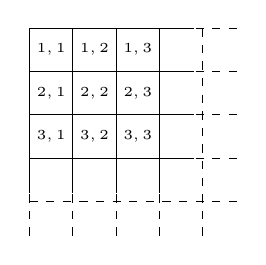
\begin{tikzpicture}[rotate=-90, scale=.55]
        \draw (1, 1) grid (4.8, 4.8);
        \draw[dashed] (1, 1) grid (5.8, 5.8);
        \foreach \i in {1, 2, 3} {
                \foreach \j in {1, 2, 3} {
                        \draw (\i, \j) rectangle (\i + 1, \j + 1) node[pos=.5] {\tiny \(\i, \j\)};
                    }
            }
    \end{tikzpicture}
    \caption{The set \(\positives^2\), with its elements graphically represented as unit boxes in the plane. The elements of the subset \(\interval{3}^2 \subset \positives^2\) are labeled with their coordinates.}
    \label{fig:positives2}
\end{figure}

The set \(\positives^2\) is partitioned into \vocab{rows}, where the \(i\)\textsuperscript{th} row is the set \(\{i\} \times \positives\),
and also partitioned into \vocab{columns}, where the \(j\)\textsuperscript{th} column is the set \(\positives \times \{j\}\).

\newcommand\coordleq{\leq_\mathrm{coord}}

The \vocab{coordinatewise partial order} on \(\positives^2\) is the partial order \(\coordleq\) given by
\begin{equation*}
    (i, j) \coordleq (i', j') \qquad \text{if and only if} \qquad i \leq i' \quad \text{and} \quad j \leq j'.
\end{equation*}
See Figure~\ref{fig:coordleq} for a graphical representation of the coordinatewise partial order \(\coordleq\) on \(\positives^2\).

\begin{figure}[htbp]
    \centering
    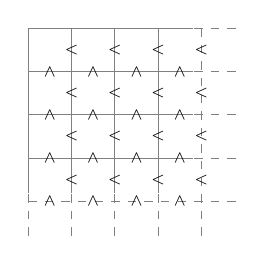
\begin{tikzpicture}[rotate=-90, scale=.55]
        \draw[black!50] (1, 1) grid (4.8, 4.8);
        \draw[black!50, dashed] (1, 1) grid (5.8, 5.8);
        \foreach \i in {1, 2, 3, 4} {
                \foreach \j in {1, 2, 3, 4} {
                        \node at (\i + .5, \j + 1) {\tiny \(<\)};
                    }
            }
        \foreach \i in {1, 2, 3, 4} {
                \foreach \j in {1, 2, 3, 4} {
                        \node[rotate=-90] at (\i + 1, \j + .5) {\tiny \(<\)};
                    }
            }
    \end{tikzpicture}
    \caption{The set \(\positives^2\), with its elements ordered by the coordinatewise partial order \(\coordleq\).
        Although only the relations between adjacent elements are shown, the relation between an arbitrary pair of elements is determined by the transitivity of the relations in the figure.}
    \label{fig:coordleq}
\end{figure}

A \vocab{Young diagram} is a diagram \(D \subset \positives^2\) such that, if \((i, j) \in D\), then \((i', j') \in D\) for all \((i', j') \coordleq (i, j)\).
Given a partition \(\lambda\), \vocab{the Young diagram of the partition} \(\lambda\) is the subset of \(\positives^2\) given by
\begin{equation*}
    \left\{ (i, j) \in \positives^2 \ : \  j \leq \lambda_i \right\}.
\end{equation*}
For example, the Young diagram of \(\composition{3, 3, 1}\) is the subset of \(\positives^2\) given by
\begin{equation*}
    \Big\{ (1, 1), (1, 2), (1, 3), \quad (2, 1), (2, 2), (2, 3), \quad (3, 1) \Big\},
\end{equation*}
which is graphically represented in Figure~\ref{fig:youngdiagram}.

\begin{figure}[htbp]
    \centering
    \ydiagram{3, 3, 1}
    \caption{The Young diagram of the partition \(\composition{3, 3, 1}\).}
    \label{fig:youngdiagram}
\end{figure}

As an abuse of notation, we use \(\lambda\) to denote both the partition and its Young diagram.

\section{Counting Vector Spaces}

\begin{definition}[Grassmanian]
    Let \(\mathbb{K}\) be a field,
    \(V\) be a vector space over \(\mathbb{K}\),
    and \(d \in \nonnegatives\).
    The \vocab{Grassmannian} \(\Grassmanian_d(V)\) is the set of all \(d\)-dimensional subspaces of \(V\).
\end{definition}

\begin{definition}
    The \vocab{\(q\)-binomial coefficient}, or \vocab{Gaussian coefficient}, is
    \[
        \qbinom{n}{k} = \prod_{i=0}^{k-1} \frac{1 - q^{n-i}}{1 - q^{k-i}}.
    \]
\end{definition}

\begin{proposition}[\(q\)-binomial coefficient recursion]
    For all \(n, k \in \positives\),
    \[
        \qbinom{n}{k} =
        \begin{cases}
            1 & \text{if } k = 0 \text{ or } k = n, \\    
            \qbinom{n-1}{k} + q^{n-k} \qbinom{n-1}{k-1} & \text{otherwise}.
        \end{cases}
    \]
\end{proposition}

\begin{corollary}
    The \(q\)-binomial coefficient is a polynomial in \(q\) with nonnegative integer coefficients.
\end{corollary}

\begin{corollary}
    For all \(n, k \in \positives\),
    \[
        \qbinom[1]{n}{k} = \binom{n}{k}.
    \]
\end{corollary}

\begin{lemma} \label{lem:grassmanian_qbinomial_prime_power}
    Let \(p\) be a prime, \(m \in \positives\), and \(\ell, w \in \nonnegatives\).
    Let \(q = p^m\).
    Then,
    \[
        \qbinom{\ell + w}{\ell}
        = \left|
            \Grassmanian_\ell\left(\finitefield{q}^{\ell + w} \right)
        \right|
        = \sum{\lambda \in \Par_{\ell, w}} (q)^{|\lambda|}.
    \]
\end{lemma}

\begin{proof}[Proof of the first equality.]
    Let \(\mathcal{M}\) be the set of all \(\ell \times (\ell + w)\) matrices with entries in \(\finitefield{q}\) with linearly independent rows.

    On one hand, we may count the elements of \(\mathcal{M}\) by choosing the \(\ell\) linearly independent rows one by one.
    There are \(q^{\ell + w} - 1\) choices for the first row,
    \(q^{\ell + w} - q\) choices for the second row, and so on.
    In general, there are \(q^{\ell + w} - q^{i-1}\) choices for the \(i\)\textsuperscript{th} row.
    Therefore,
    \begin{equation*}
        \left|
            \mathcal{M}
        \right|
        = \prod_{i=1}^{\ell} (q^{\ell + w} - q^{i-1})
    \end{equation*}

    On the other hand, we may count the elements of \(\mathcal{M}\) by first choosing the linear span of its rows, and then choosing the rows themselves in such linear span.
    There are \(|\Grassmanian_\ell(\finitefield{q}^{\ell + w})|\) choices for an \(\ell\)-dimensional subspace of \(\finitefield{q}^{\ell + w}\).
    Given such a subspace,
    there are \(q^{\ell} - 1\) choices for the first row,
    there are \(q^{\ell} - q\) choices for the second row, and so on.
    In general, there are \(q^{\ell} - q^{i-1}\) choices for the \(i\)\textsuperscript{th} row.
    Therefore,
    \begin{equation*}
        \left|
            \mathcal{M}
        \right|
        = \left|
            \Grassmanian_\ell\left(\finitefield{q}^{\ell + w} \right)
        \right|
        \prod_{i=1}^{\ell} (q^{\ell} - q^{i-1})
    \end{equation*}

    Finally, from the two expressions for \(\left| \mathcal{M} \right|\), we find
    \begin{align*}
        \left|
            \Grassmanian_\ell\left(\finitefield{q}^{\ell + w} \right)
        \right|
        = \prod_{i=1}^{\ell} \frac{q^{\ell + w} - q^{i-1}}{q^{\ell} - q^{i-1}} \\
        = \prod_{i=0}^{\ell - 1} \frac{1 - q^{\ell + w - i}}{1 - q^{\ell - i}} \\
        = \qbinom{\ell + w}{\ell},
    \end{align*}
    as desired for the first equality.
\end{proof}

\begin{proof}[Proof for the second equality]
    By linear algebra, the \(\Grassmanian_\ell(\finitefield{q}^{\ell + w})\) is in bijection with the set of \(\ell \times (\ell + w)\) matrices with independent rows and in row reduced echelon form.

    The set of \(\ell \times (\ell + w)\) matrices with independent rows and in row reduced echelon form is in bijection with the set of partitions of \(\ell\) with at most \(w\) parts by the following correspondence:
    \begin{quote}
        ``Start from the \(\ell \times (\ell + w)\) matrix with independent rows and in row reduced echelon form.
        There are \(\ell\) pivots, one in each row.
        Delete all zeroes southwest of the pivots, and delete all \(\ell\) pivot columns.
        The resulting matrix-looking table of elements of \(\finitefield{q}\) can be interpreted as an assignment of elements of \(\finitefield{q}\) to the boxes of the Young diagram within the rectangle of size \(\ell \times w\).''
    \end{quote}

    Note that, for each Young diagram within the rectangle of size \(\ell \times w\), there are \(q^{|\lambda|}\) ways to assign elements of \(\finitefield{q}\) to the boxes of the Young diagram.
    Therefore,
    \[
        \left|
            \Grassmanian_\ell\left(\finitefield{q}^{\ell + w} \right)
        \right|
        = \sum_{\lambda \in \Par_{\ell, w}} (q)^{|\lambda|},
    \]
    as desired for the second equality.
\end{proof}

\begin{theorem}
    Let \(\ell, w \in \nonnegatives\).
    Then,
    \[
        \sum_{\lambda \in \Par_{\ell, w}} q^{|\lambda|}
        = \qbinom{\ell + w}{\ell}.
    \]
\end{theorem}

\begin{proof}
    From Lemma~\ref{lem:grassmanian_qbinomial_prime_power},
    we know that the two polynomials agree at prime powers.
    Since the two polynomials agree at infinitely many points,
    they must be equal.
\end{proof}

\begin{definition}[Schubert cell]
    Let \(\lambda\) be a partition.
    Let \(V\) be a vector space of dimension \(d\), and let \(k\) be an integer such that \(0 \leq k \leq d\).
    The \vocab{Schubert cell} \(X^\circ_\lambda\) (of \(V\)) is the set of all \(k\)-dimensional subspaces of \(V\) such that \(\lambda\) is the Young diagram obtained from the unique \(k \times d\).
\end{definition}
    \chapter{Permutations}

Let \(n\) be a non-negative integer.
The \vocab{\(n\)\textsuperscript{th} symmetric group} \(\sym_n\)
is the group of bijections from \(\{1, 2, \ldots, n\}\) to itself,
under composition.
A permutation \(w \in \sym_n\) can be written in \vocab{two-line notation} as
\[
    \begin{pmatrix}
        1    & 2    & \cdots & n    \\
        w(1) & w(2) & \cdots & w(n)
    \end{pmatrix},
\]
or in \vocab{one-line notation} as
\[
    w(1)w(2)\cdots w(n).
\]
We may also think of a permutation \(w \in \sym_n\) as a directed graph with vertex set \(\{1, 2, \ldots, n\}\) and edges \(\{(i, w(i)) \mid i = 1, \ldots, n\}\). The connected components of this graph are cycles.


Each permutation \(w\) has an associated partition \(\cyc(w) \vdash n\) whose parts are the lengths of the cycles of \(w\), called the \vocab{cycle type} of \(w\). It is known that \(\cyc(w) = \cyc(u)\) if and only if \(w\) and \(u\) are conjugate in \(\sym_n\). Thus, the conjugacy class corresponding to a partition \(\lambda \vdash n\) is
\[
    \zeta_\lambda = \{ w \in \sym_n \mid \cyc(w) = \lambda \}.
\]

The centralizer of \(w \in \sym_n\) is
\[
    Z(w) = \{ u \in \sym_n \mid uw = wu \}.
\]
Let \(\lambda\) be a partition of \(n\), and let \(j_i\) be the number of parts of \(\lambda\) equal to \(i\). For \(w \in \zeta_\lambda\), the size of the centralizer is
\[
    |Z(w)| = \prod_{i=1}^n (j_i)! \prod_{k=1}^{\ell(\lambda)} \lambda_k,
\]
which does not depend on the choice of \(w \in \zeta_\lambda\). We denote this expression by \(z_\lambda\). Moreover, the size of the conjugacy class is
\[
    |\zeta_\lambda| = \frac{n!}{z_\lambda}.
\]

A permutation \(w \in \sym_n\) is called a \vocab{transposition} if \(\cyc(w) = 2\,1^{n-2}\), meaning \(w\) swaps two elements and fixes the rest. A \vocab{simple transposition} is a transposition of the form \(\eltr{i} = (i, i+1)\) for some \(i \in \{1, \ldots, n-1\}\).

The symmetric group \(\sym_n\) is generated by the simple transpositions \(\eltr{1}, \eltr{2}, \ldots, \eltr{n-1}\), subject to the relations:
\begin{align*}
    \eltr{i}^2                 & = 1,                                           \\
    \eltr{i}\eltr{j}           & = \eltr{j}\eltr{i} \quad \text{if } |i-j| > 1, \\
    \eltr{i}\eltr{i+1}\eltr{i} & = \eltr{i+1}\eltr{i}\eltr{i+1}.
\end{align*}
Groups with presentations similar to this one are called \vocab{Coxeter groups}.

Given a permutation \(w \in \sym_n\), an \vocab{inversion} is a pair \((i, j)\) such that \(i < j\) and \(w(i) > w(j)\). The number of inversions of \(w\) is denoted by \(\inv(w)\). The \vocab{Coxeter length} of \(w\) is the minimum number of simple transpositions needed to express \(w\) and equals \(\inv(w)\).

The \vocab{sign} of a permutation \(w\) is defined as \(\sign(w) = (-1)^{\inv(w)}\). This function \(\sign \colon \sym_n \to \{\pm 1\}\) is a group homomorphism. For \(w \in \zeta_\lambda\), we have \(\sign(w) = (-1)^{n - \ell(\lambda)}\), where \(\ell(\lambda)\) is the number of parts in \(\lambda\).

The symmetric group \(\sym_n\) has a unique element of minimum inversion number, namely the identity permutation \(\id\) with \(\inv(\id) = 0\), and a unique element of maximum inversion number, the permutation \(\omega_0 = n\, (n-1)\, \ldots\, 1\) with \(\inv(\omega_0) = \binom{n}{2}\).

For \(w \in \sym_n\), the \vocab{permutation matrix} \(M(w) \in \GL_n(\mathbb{C})\) is defined by \(M(w)_{ij} = \delta_{i, w(j)}\). The map \(M \colon \sym_n \to \GL_n(\mathbb{C})\) is a group homomorphism, and \(\sign\) equals the composition \(\det \circ M\).

A \vocab{(linear) representation} of a group \(G\) is a group homomorphism \(\rho \colon G \to \GL_n(\mathbb{C})\) for some \(n\). For example, \(M \colon \sym_n \to \GL_n(\mathbb{C})\) is a representation. A \vocab{permutation representation} of \(G\) is a homomorphism \(\rho \colon G \to \sym_n\) for some \(n\). Given any permutation representation \(\rho \colon G \to \sym_n\), composing with \(M\) yields a linear representation \(\rho' \colon G \to \GL_n(\mathbb{C})\).

Given a set \(S\) and a group action \(\rho \colon G \to \sym(S)\), the \vocab{fixed set} of \(S\) under \(\rho\) is
\[
    S^G = \{ s \in S \mid \rho(g)(s) = s \text{ for all } g \in G \}.
\]
Similarly, if \(V\) is a vector space with a representation \(\rho \colon G \to \GL(V)\), the \vocab{invariant subspace} is
\[
    V^G = \{ v \in V \mid \rho(g)v = v \text{ for all } g \in G \}.
\]
One can view \(V^G\) as the intersection of the eigenspaces associated with the eigenvalue \(1\) of the matrices \(\rho(g)\) for all \(g \in G\).

As an example, let \(\mathcal{G}_n\) be the set of all graphs on the vertex set \(\{1, 2, \ldots, n\}\). The group \(\sym_n\) acts on \(\mathcal{G}_n\) by permuting vertices: for \(w \in \sym_n\) and \(G \in \mathcal{G}_n\), the graph \(w \cdot G\) is obtained by applying \(w\) to the vertices of \(G\). Under this action, the only fixed graphs are the empty graph and the complete graph.

An \vocab{action of a group \(G\) on a ring \(R\)} is a group homomorphism \(\rho \colon G \to \Aut(R)\), where \(\Aut(R)\) is the group of ring automorphisms of \(R\). The fixed set \(R^G\) is a subring of \(R\).

An \vocab{algebra over a field \(k\)} is a vector space \(A\) over \(k\) equipped with a bilinear multiplication \(\cdot \colon A \times A \to A\). If \(A\) is a \(k\)-algebra, it contains a copy of \(k\) as a subring. Conversely, if \(A\) is a ring containing a field \(k\) as a subring, then \(A\) is a \(k\)-algebra.

Examples of \(k\)-algebras include the ring of polynomials \(k[x]\), the ring of power series \(k[[x]]\), and the ring of matrices \(\Mat_n(k)\).

Given \(k\)-algebras \(A\) and \(B\), a \vocab{\(k\)-algebra homomorphism} is a map \(\varphi \colon A \to B\) that is both a ring homomorphism and \(k\)-linear. An \vocab{action of a group \(G\) on a \(k\)-algebra \(A\)} is a group homomorphism \(\rho \colon G \to \Aut(A)\), where \(\Aut(A)\) is the group of \(k\)-algebra automorphisms of \(A\). The fixed set \(A^G\) is a \(k\)-subalgebra of \(A\).

A \vocab{monomial} is a product of powers of variables. In \(\mathbb{Q}[x_1, x_2, \ldots, x_n]\), monomials are indexed by \(\mathbb{N}^n\):
\[
    x^\alpha = x_1^{\alpha_1}x_2^{\alpha_2}\cdots x_n^{\alpha_n},
\]
for \(\alpha = (\alpha_1, \alpha_2, \ldots, \alpha_n) \in \mathbb{N}^n\). The \vocab{degree} of \(x^\alpha\) is \(\deg(x^\alpha) = \alpha_1 + \alpha_2 + \cdots + \alpha_n\). The set of monomials forms a basis for \(\mathbb{Q}[x_1, x_2, \ldots, x_n]\) as a vector space over \(\mathbb{Q}\).

We denote by \(\mathbb{Q}[x_1, x_2, \ldots, x_n]_d\) the subspace spanned by monomials of degree \(d\), giving the direct sum decomposition
\[
    \mathbb{Q}[x_1, x_2, \ldots, x_n] = \bigoplus_{d=0}^\infty \mathbb{Q}[x_1, x_2, \ldots, x_n]_d.
\]

The group \(\sym_n\) acts on monomials by
\[
    w \cdot x^\alpha = x^{w(\alpha)} = x_{w^{-1}(1)}^{\alpha_1}x_{w^{-1}(2)}^{\alpha_2}\cdots x_{w^{-1}(n)}^{\alpha_n}.
\]
This action extends linearly to \(\mathbb{Q}[x_1, x_2, \ldots, x_n]\). The \vocab{algebra of symmetric polynomials} is the subalgebra \(\Sym_n = \mathbb{Q}[x_1, x_2, \ldots, x_n]^{\sym_n}\) consisting of all polynomials fixed under this action.

    \chapter{Symmetric Functions}

Let \(\sym_\infty\) be the group of bijections from \(\nonnegatives\) to itself that fix all but finitely many elements, under composition.
Let \(\rationals[[x_1, x_2, \ldots]]_{\mathsf{gr}}\)
be the subalgebra consisting of the power series in \(x_1, x_2, \ldots\)
of bounded degree.

For example,
\begin{align*}
    x_1 + x_2 + x_3 + \cdots                   & \in \rationals[[x_1, x_2, \ldots]]_{\mathsf{gr}}, \\
    x_1x_2 + x_1x_3 + \cdots + x_2x_3 + \cdots & \in \rationals[[x_1, x_2, \ldots]]_{\mathsf{gr}},
\end{align*}
but
\begin{align*}
    x_1 + x_1^2 + x_1^3 + \cdots \notin \rationals[[x_1, x_2, \ldots]]_{\mathsf{gr}},
    x_1x_2x_3x_4\cdots \notin \rationals[[x_1, x_2, \ldots]]_{\mathsf{gr}}.
\end{align*}

Note that \(\rationals[[x_1, x_2, \ldots]]_{\mathsf{gr}}\) is a graded \(\rationals\)-algebra,
however its homogeneous components are infinite-dimensional,
hence it has no Hilbert series.

\begin{definition}
    The \vocab{algebra of symmetric functions} is
    \[
        \Sym = \rationals[[x_1, x_2, \ldots]]_{\mathsf{gr}}^{\sym_\infty},
    \]
\end{definition}

Note that there are projections \(\Sym(n) \to \Sym(n-1)\) for all \(n\),
where \(x_n\) is sent to \(0\) and the other variables are fixed.
Thus, we have a sequence of maps
\[
    \cdots \to \Sym(n) \to \Sym(n-1) \to \cdots \to \Sym(2) \to \Sym(1) \to \rationals,
\]
and the algebra of symmetric functions \(\Sym\) is the inverse limit of this sequence; whatevers that means.

There is a projection \(\Sym \to \Sym(n)\) that sends \(x_i\) to \(0\) for all \(i > n\), and the other variables are fixed.

Given a partition \(\lambda \in \Par\),
the \vocab{monomial symmetric function} \(m_\lambda \in \Sym\) is defined by
\[
    m_\lambda = \sum_{\sort{\alpha} = \lambda} x^\alpha.
\]
The set of monomial symmetric functions
\[
    \{ m_\lambda \mid \lambda \in \Par \}
\]
is a basis for \(\Sym\).

Any formula that holds in \(\Sym\) will hold in \(\Sym(n)\) after sending \(m_\lambda\) to \(m_\lambda(x_1, x_2, \ldots, x_n)\) if \(\ell(\lambda) \leq n\), and to \(0\) otherwise.
In some sense, the converse of this statement is also true: any formula that holds in \(\Sym(n)\) for all \(n\) will hold in \(\Sym\).

We might also want to define the \vocab{formal completion} of \(\Sym\) as
\begin{equation*}
    \widehat\Sym = \rationals[[x_1, x_2, \ldots]]^{\sym_\infty}.
\end{equation*}
For example,
\begin{equation*}
    m_1 + m_2 + m_3 + \cdots \in \widehat\Sym.
\end{equation*}

Back to the algebra of symmetric functions,
\(\Sym\) is a graded \(\rationals\)-algebra,
where the homogeneous component of degree \(d\) is \(\Sym_d\).
The dimension of \(\Sym_d\) is the number of partitions of \(d\),
and therefore the Hilbert series of \(\Sym\) is
\begin{equation*}
    \Hilb(\Sym; t) = \prod_{i=1}^\infty \frac{1}{1-t^i}.
\end{equation*}

Consider \(N = \rationals[x_1, x_2, \ldots]\), the ring of polynomials in infinitely many variables, which is also a graded \(\rationals\)-algebra.
But \(\dim N_1 = \infty\), so \(N\) has no Hilbert series.
Consider \(N' = N\) with nonstandard grading where \(\deg(x_i) = i\) for all \(i \in \nonnegatives\).
Then, \(\dim N'_d\) is the number of partitions of \(d\), so
\begin{equation*}
    \Hilb(N'; t) = \prod_{i=1}^\infty \frac{1}{1-t^i} = \Hilb(\Sym; t).
\end{equation*}
This makes us expect that \(\Sym\) to look like \(N'\).

How do we explain this? We find generators of \(\Sym\), one in each degree, with no relations between them.
There are three simple answers to this question:
\begin{itemize}
    \item \vocab{power sum symmetric functions} \(p_k = \sum_{i=1}^\infty x_i^k\),
    \item \vocab{elementary symmetric functions} \(e_k = \sum_{1 \leq i_1 < i_2 < \cdots < i_k} x_{i_1}x_{i_2}\cdots x_{i_k}\),
    \item \vocab{complete homogeneous symmetric functions} \(h_k = \sum_{1 \leq i_1 \leq i_2 \leq \cdots \leq i_k} x_{i_1}x_{i_2}\cdots x_{i_k}\).
\end{itemize}

\section{Power Sum Symmetric Functions}

The \vocab{\(n\)\textsuperscript{th} power sum symmetric function \(p_n \in \Sym\)} is defined by
\begin{equation}
    p_n = \sum_{i=1}^\infty x_i^n.
\end{equation}
Given a partition \(\lambda \in \Par\), define \(p_\lambda = p_{\lambda_1}p_{\lambda_2}\cdots p_{\lambda_{\ell(\lambda)}}\).

\begin{theorem} \label{thm:pn_sym}
    The four following statements are true:
    \begin{enumerate}
        \item \label{item:pl_symd_basis}
              The set \(\{p_\lambda : \lambda \in \Par(d)\}\) forms a basis for \(\Sym_d\).
        \item \label{item:pl_sym_basis}
              The set \(\{p_\lambda : \lambda \in \Par\}\) forms a basis for \(\Sym\).
        \item \label{item:pn_sym_generates}
              The set \(\{p_i : i \in \positives\}\) generates \(\Sym\) and is algebraically independent.
        \item \label{item:pn_sym_graded_isom}
              The map \(N' \to \Sym\) obtained by the extension of the map \(x_i \mapsto p_i\) is an isomorphism of graded \(\rationals\)-algebras.
    \end{enumerate}
\end{theorem}

\begin{example}[Theorem~\ref{thm:pn_sym}\ref{item:pl_symd_basis} for \(d = 3\)]
    There are three partitions of \(3\), namely \(\composition{3}\), \(\composition{2, 1}\), and \(\composition{1, 1, 1}\).
    The corresponding power sum symmetric functions are
    \begin{align*}
        p_{\composition{3}}       & = p_3 = x_1^3 + x_2^3 + x_3^3 + \cdots,                                \\
        p_{\composition{2, 1}}    & = p_2p_1 = (x_1^2 + x_2^2 + x_3^2 + \cdots)(x_1 + x_2 + x_3 + \cdots), \\
        p_{\composition{1, 1, 1}} & = p_1^3 = (x_1 + x_2 + x_3 + \cdots)^3,
    \end{align*}
    which can be expanded in terms of monomial symmetric functions as
    \begin{align*}
        p_{\composition{3}}       & = m_{\composition{3}}                                                         \\
        p_{\composition{2, 1}}    & = m_{\composition{3}} + m_{\composition{2, 1}}                                \\
        p_{\composition{1, 1, 1}} & = m_{\composition{3}} + 3m_{\composition{2, 1}} + 6m_{\composition{1, 1, 1}}.
    \end{align*}
    Hence,
    \begin{equation*}
        \begin{bsmallmatrix}
            p_{\composition{1, 1, 1}} \\ p_{\composition{2, 1}} \\ p_{\composition{3}}
        \end{bsmallmatrix}
        =
        \begin{bsmallmatrix}
            6 & 3 & 1 \\
            0 & 1 & 1 \\
            0 & 0 & 1
        \end{bsmallmatrix}
        \begin{bsmallmatrix}
            m_{\composition{1, 1, 1}} \\ m_{\composition{2, 1}} \\ m_{\composition{3}}
        \end{bsmallmatrix}.
    \end{equation*}
    Since
    \(
    \begin{bsmallmatrix}
        6 & 3 & 1 \\
        0 & 1 & 1 \\
        0 & 0 & 1
    \end{bsmallmatrix}
    \)
    is an invertible matrix and \(\{m_{\composition{3}}, m_{\composition{2, 1}}, m_{\composition{1, 1, 1}}\}\) is a basis for \(\Sym_3\),
    it follows that \(\{p_{\composition{3}}, p_{\composition{2, 1}}, p_{\composition{1, 1, 1}}\}\) is a basis for \(\Sym_3\).

    Note that \(\{p_{\composition{3}}, p_{\composition{2, 1}}, p_{\composition{1, 1, 1}}\}\) is \emph{not} a \(\mathbb{Z}\)-basis for the integer symmetric functions, as the matrix has determinant \(6\).
\end{example}

\begin{proof}[Proof of Theorem~\ref{thm:pn_sym}(a)]
    Let \(d\) be an integer and \(\lambda \in \Par(d)\).
    Note that
    \begin{align*}
        p_\lambda
         & = p_{\lambda_1}p_{\lambda_2}\cdots p_{\lambda_{\ell(\lambda)}}            \\
         & = \left( \prod_i j_i! \right) m_\lambda + \sum_{\substack{\mu \in \Par(d) \\ \lambda \lessref \mu}} R_{\lambda\mu}m_\mu,
    \end{align*}
    where \(R_{\lambda\mu}\) are positive integers.%
    \footnote{A future homework problem might ask to compute \(R_{\lambda\mu}\).}
    Take a total order that extends the refinement order on \(\Par(d)\), and write two vectors \((p_\lambda)\) and \((m_\lambda)\) in this order.
    Then, the matrix that maps \((\mu_\lambda)\) to \((p_\lambda)\) is upper triangular with positive diagonal entries, hence invertible.
    Finally, since \(\{m_\lambda : \lambda \in \Par(d)\}\) is a basis for \(\Sym_d\), it follows that \(\{p_\lambda : \lambda \in \Par(d)\}\) is a basis for \(\Sym_d\).
\end{proof}

Note that the \(p\)-basis is \(m\)-positive, i.e., the coefficients of the \(p\)-basis in the \(m\)-basis are nonnegative integers,
and \(m\)-integral, i.e., the coefficients of the \(p\)-basis in the \(m\)-basis are integers.

\section{Elementary Symmetric Functions}

The \vocab{\(n\)\textsuperscript{th} elementary symmetric function \(e_n \in \Sym\)} is defined by
\begin{equation}
    e_n = \sum_{1 \leq i_1 < i_2 < \cdots < i_n} x_{i_1}x_{i_2}\cdots x_{i_n}.
\end{equation}
Given a partition \(\lambda \in \Par\), define \(e_\lambda = e_{\lambda_1}e_{\lambda_2}\cdots e_{\lambda_{\ell(\lambda)}}\).

\begin{theorem}[Fundamental Theorem of Symmetric Functions] \label{thm:en_sym}
    The four following statements are true:
    \begin{enumerate}
        \item \label{item:el_symd_basis}
              The set \(\{e_\lambda : \lambda \in \Par(d)\}\) forms a basis for \(\Sym_d\).
        \item \label{item:el_sym_basis}
              The set \(\{e_\lambda : \lambda \in \Par\}\) forms a basis for \(\Sym\).
        \item \label{item:en_sym_generates}
              The set \(\{e_i : i \in \positives\}\) generates \(\Sym\) and is algebraically independent.
        \item \label{item:en_sym_graded_isom}
              The map \(N' \to \Sym\) obtained by the extension of the map \(x_i \mapsto e_i\) is an isomorphism of graded \(\rationals\)-algebras.
    \end{enumerate}
\end{theorem}

A \vocab{contingency table} is a function \(A \colon \positives \times \positives \to \nonnegatives\) such that all but finitely many entries are non-zero.
Let \(\operatorname{row}(A)\) be the sequence of row sums of \(A\),
and let \(\operatorname{col}(A)\) be the sequence of column sums of \(A\).
Note that the sum of \(\operatorname{row}(A)\) is equal to the sum of \(\operatorname{col}(A)\), hence they are weak compositions of the same integer.
See Figure~\ref{fig:contingency_table} for an example of a contingency table.

\begin{figure}[htbp]
	\begin{equation*}
		\arraycolsep=7pt
		\def\arraystretch{1.3}
		\begin{array}{c|ccccc}
			& \textcolor{red}{4} & \textcolor{red}{6} & \textcolor{red}{5} & \textcolor{red}{0} & \cdots \\ \hline
			\textcolor{red}{6} & 1      & 4      & 3      & 0      & \cdots \\
			\textcolor{red}{3} & 0      & 2      & 1      & 0      & \cdots \\
			\textcolor{red}{4} & 3      & 0      & 1      & 0      & \cdots \\
			\textcolor{red}{0} & 0      & 0      & 0      & 0      & \cdots \\
			\vdots             & \vdots & \vdots & \vdots & \vdots & \ddots
		\end{array}
	\end{equation*}
	\caption{A contingency table (in black) \(A\) with \(\operatorname{row}(A) = \composition{6, 3, 4}\) and \(\operatorname{col}(A) = \composition{4, 6, 5}\) (in red).}
	\label{fig:contingency_table}
\end{figure}

Given weak compositions \(\alpha, \beta\),
let \(M_{\alpha\beta}\) be the number of contingency tables with entries in \(\{0, 1\}\) such that \(\operatorname{row}(A) = \alpha\) and \(\operatorname{col}(A) = \beta\).

We start with some facts about \(M_{\alpha\beta}\), which are used later without reference.

\begin{fact} \label{fact:Mab-same-sum}
	If \(\alpha, \beta\) are weak compositions of different integers, then \(M_{\alpha\beta} = 0\).
\end{fact}
\begin{proof}
	If \(A\) is a contingency table with \(\operatorname{row}(A) = \alpha\) and \(\operatorname{col}(A) = \beta\),
	then the sum of \(\alpha\) is equal to the sum of \(\beta\) because both are equal to the sum of all entries of \(A\).
\end{proof}

\begin{fact} \label{fact:Mab-Mba}
	For any weak compositions \(\alpha, \beta\),
	\(M_{\alpha\beta} = M_{\beta\alpha}\).
\end{fact}
\begin{proof}
	Reflection by the main diagonal of a contingency table is a bijection between the objects counted by \(M_{\alpha\beta}\) and \(M_{\beta\alpha}\).
\end{proof}

\begin{fact} \label{fact:Mab-rearrangement}
	If \(\alpha\) is a rearrangement of \(\alpha'\) and \(\beta\) is a rearrangement of \(\beta'\),
	then \(M_{\alpha\beta} = M_{\alpha'\beta'}\).
\end{fact}
\begin{proof}
	Let \(w\) be the permutation that rearranges \(\alpha\) to \(\alpha'\).
	The map that sends a contingency table \(A\) to another contingency table \(A'\) by applying \(w\) to the rows of \(A\) is a bijection between the objects counted by \(M_{\alpha\beta}\) and \(M_{\alpha'\beta}\).
	Applying the same argument to the columns shows that \(M_{\alpha\beta} = M_{\alpha'\beta'}\), as desired.
\end{proof}

\begin{corollary} \label{cor:Mab-Mlm}
	If \(\alpha\) is a rearrangement of a partition \(\lambda\) and \(\beta\) is a rearrangement of a partition \(\mu\),
	then \(M_{\alpha\beta} = M_{\lambda\mu}\).
\end{corollary}

Define the weight of a contingency table \(A\) to be the monomial
\begin{equation}
	\operatorname{wt}(A)
	= \prod_{i, j \geq 1} (x_iy_j)^{A(i, j)}
	= x^{\operatorname{row}(A)}y^{\operatorname{col}(A)},
\end{equation}

\begin{lemma} \label{lem:generating-function-01-contingency-tables-compositions}
	Let \(x = (x_1, x_2, \ldots)\) and \(y = (y_1, y_2, \ldots)\) be sequences of variables.
	Then,
	\begin{equation}
		\prod_{i, j \geq 1} (1 + x_iy_j)
		= \sum_{\substack{\text{contingency tables } A \\ \text{with entries in } \{0, 1\}}} \operatorname{wt}(A)
		= \sum_{\substack{\text{weak compositions} \\ \alpha, \beta}} M_{\alpha\beta} x^\alpha y^\beta.
	\end{equation}
\end{lemma}

\begin{proof}
Note that each monomial in the expansion of the power series
\begin{equation}
	\prod_{i, j \geq 1} (1 + x_iy_j)
	= \prod_{i, j \geq 1} \left( (x_iy_j)^0 + (x_iy_j)^1 \right)
\end{equation}
corresponds to a choice of \(0\) or \(1\) for the exponent of each \(x_iy_j\), which corresponds to a contingency table with entries in \(\{0, 1\}\).
Therefore,
\begin{equation}
	\prod_{i, j \geq 1} (1 + x_iy_j)
	= \sum_{\substack{\text{contingency tables } A \\ \text{with entries in } \{0, 1\}}} \operatorname{wt}(A) 
	= \sum_{\substack{\text{weak compositions} \\ \alpha, \beta}} M_{\alpha\beta} x^\alpha y^\beta, 
\end{equation}
where the last equation is obtained by computing the coefficient of each monomial.
\end{proof}

\begin{proposition} \label{prop:generating-function-01-contingency-tables-partitions}
	Let \(x = (x_1, x_2, \ldots)\) and \(y = (y_1, y_2, \ldots)\) be sequences of variables.
	Then,
	\begin{equation}
		\prod_{i, j \geq 1} (1 + x_iy_j) = \sum_{\substack{\text{partitions} \\ \lambda, \mu}} M_{\lambda\mu} m_\lambda(x) m_\mu(y).
	\end{equation}
\end{proposition}

\begin{proof}
	We have
\begin{equation}
	\prod_{i, j \geq 1} (1 + x_iy_j)
	= \sum_{\substack{\text{weak compositions} \\ \alpha, \beta}} M_{\alpha\beta} x^\alpha y^\beta
	= \sum_{\substack{\text{partitions} \\ \lambda, \mu}} M_{\lambda\mu} m_\lambda(x) m_\mu(y),
\end{equation}
where the first equality is by Lemma~\ref{lem:generating-function-01-contingency-tables-compositions},
and the second equality is obtained by collecting all monomials whose exponents are rearrangements of the same partition.
\end{proof}

\begin{proposition} \label{prop:el-expansion-in-m-basis}
	Let \(\lambda\) be a partition.
	Then,
	\begin{equation}
		e_\lambda = \sum_{\text{partitions } \mu} M_{\lambda\mu} m_\mu.
	\end{equation}
\end{proposition}

\begin{proof}
	Note that 
	\begin{equation}
		e_k(x)
		= \sum_{\substack{\{0, 1\}\text{-sequences } \alpha \\ \text{with sum } k}}
			x^\alpha
	\end{equation}
	Hence,
	\begin{align}
		e_\lambda(x)
		= \prod_{i\geq 1} e_{\lambda_i}
		&= \prod_{i\geq 1}
			\sum_{\substack{\text{weak compositions } \alpha \\ \text{with entries in } \{0, 1\} \\ \text{and sum } \lambda_i}}
				x^{\alpha^{(i)}} \\
		&= \sum_{\substack{\text{contingency tables } A \\ \text{with entries in } \{0, 1\} \\ \text{and column sum } \lambda}}
			x^{\operatorname{row}(A)}.
	\end{align}
	By Lemma~\ref{lem:generating-function-01-contingency-tables-compositions},
	\(e_\lambda(x)\) is the coefficient of \(y^\lambda\) in \(\prod_{i, j \geq 1} (1 + x_iy_j)\) as a power series in \(y\) with coefficients in \(\rationals[[x_1, x_2, \ldots]]\),
	that is,
	\begin{equation}
		e_\lambda(x) = \sum_{\text{weak compositions } \alpha} M_{\alpha\lambda} x^\alpha = \sum_{\text{partitions } \mu} M_{\mu\lambda} m_\mu(x),
	\end{equation}
	which completes the proof.
\end{proof}

The following corollary is a direct consequence of Propositions~\ref{prop:generating-function-01-contingency-tables-partitions} and~\ref{prop:el-expansion-in-m-basis}.

\begin{corollary}
	Let \(x = (x_1, x_2, \ldots)\) and \(y = (y_1, y_2, \ldots)\) be sequences of variables.
	Let \(\lambda\) be a partition.
	Then,
	\begin{equation}
		\prod_{i, j \geq 1} (1 + x_iy_j) = \sum_{\lambda \in \Par} e_\lambda(x) m_\lambda(y).
	\end{equation}	
\end{corollary}

\begin{lemma}
    Let \(\lambda, \mu \in \Par(d)\).
    Then, \(M_{\lambda\mu} = 0\) if \(\mu \not\leq \tilde{\lambda}\),
    where \(\tilde{\lambda}\) is the conjugate of \(\lambda\).
    Moreover, \(M_{\lambda\tilde{\lambda}} = 1\).
\end{lemma}

\begin{proof}
	Suppose \(M_{\lambda\mu} \neq 0\).
	Then, there is a contingency table \(A\) with entries in \(\{0, 1\}\) such that \(\operatorname{row}(A) = \lambda\) and \(\operatorname{col}(A) = \mu\).
	Let \(B\) be the contingency table obtained by left-justifying the ones in \(A\).
	Then, \(\operatorname{row}(B) = \lambda\) and \(\operatorname{col}(B) = \tilde{\lambda}\).

	Fix \(i\).
	Note that
	\begin{align}
		\tilde{\lambda}_1 + \dots + \tilde{\lambda}_i
		 & = \text{number of ones in the first \(i\) columns of \(B\)}    \\
		 & \geq \text{number of ones in the first \(i\) columns of \(A\)}
		\geq \mu_1 + \dots + \mu_i.
	\end{align}
	Therefore, \(\tilde{\lambda} \geq \mu\).

	It is straightforward to see that \(M_{\lambda\tilde{\lambda}} = 1\), with the only possible contingency table having ones in the entries of the Young diagram of \(\lambda\) (in the English notation).
\end{proof}

\begin{proof}[Proof of Theorem~\ref{thm:en_sym}\ref{item:el_symd_basis}]
    Let \(d\) be an integer and \(\lambda \in \Par(d)\).
    Note that
    \begin{equation*}
        e_{\tilde{\lambda}}
        = m_\lambda + \sum_{\substack{\mu \in \Par(d) \\ \mu < \lambda}} M_{\lambda\mu} m_\mu.
    \end{equation*}
    Take a total order that extends the dominance order on \(\Par(d)\),
    and write two vectors \((e_{\tilde{\lambda}})\) and \((m_\lambda)\) in this order.
    Then, the matrix that maps \((m_\mu)\) to \((e_{\tilde{\lambda}})\) is upper triangular with positive diagonal entries, hence invertible.
    Finally, since \(\{m_\lambda : \lambda \in \Par(d)\}\) is a basis for \(\Sym_d\), it follows that \(\{e_{\tilde{\lambda}} : \lambda \in \Par(d)\}\) is a basis for \(\Sym_d\).

    Moreover, since the diagonal entries of the matrix are all \(1\), this matrix has an inverse with integer entries, and consequently \(\{e_{\tilde{\lambda}} : \lambda \in \Par(d)\}\) is a \(\mathbb{Z}\)-basis for the integer symmetric functions.
\end{proof}


\section{Complete Homogeneous Symmetric Functions}

The \vocab{\(n\)\textsuperscript{th} complete homogeneous symmetric function \(h_n \in \Sym\)} is defined by
\begin{equation}
    h_n = \sum_{1 \leq i_1 \leq i_2 \leq \cdots \leq i_n} x_{i_1}x_{i_2}\cdots x_{i_n}.
\end{equation}
Given a partition \(\lambda \in \Par\), define \(h_\lambda = h_{\lambda_1}h_{\lambda_2}\cdots h_{\lambda_{\ell(\lambda)}}\).

\begin{theorem} \label{thm:hn_sym}
		The four following statements are true:
		\begin{enumerate}
				\item \label{item:hl_symd_basis}
							The set \(\{h_\lambda : \lambda \in \Par(d)\}\) forms a basis for \(\Sym_d\).
				\item \label{item:hl_sym_basis}
							The set \(\{h_\lambda : \lambda \in \Par\}\) forms a basis for \(\Sym\).
				\item \label{item:hn_sym_generates}
							The set \(\{h_i : i \in \positives\}\) generates \(\Sym\) and is algebraically independent.
				\item \label{item:hn_sym_graded_isom}
							The map \(N' \to \Sym\) obtained by the extension of the map \(x_i \mapsto h_i\) is an isomorphism of graded \(\rationals\)-algebras.
		\end{enumerate}
\end{theorem}

\begin{example}[Theorem~\ref{thm:hn_sym}\ref{item:hl_symd_basis} for \(d = 3\)]
    We claim that \(\{h_{\lambda} : \lambda \in \Par(3)\}\) is a basis for \(\Lambda_3\).
    \[
        \begin{bsmallmatrix}
            h_{1,1,1} \\
            h_{2,1}   \\
            h_3
        \end{bsmallmatrix}
        =
        \begin{bsmallmatrix}
            6 & 3 & 1 \\
            3 & 2 & 1 \\
            1 & 1 & 1
        \end{bsmallmatrix}
        \begin{bsmallmatrix}
            m_{1,1,1} \\
            m_{2,1}   \\
            m_3
        \end{bsmallmatrix}.
    \]
    Since the matrix
		\(
        \begin{bsmallmatrix}
            6 & 3 & 1 \\
            3 & 2 & 1 \\
            1 & 1 & 1
        \end{bsmallmatrix}
    \)
    is invertible, \(\{h_{1,1,1}, h_{2,1}, h_3\}\) forms a basis of \(\Lambda_3\). Moreover,
		\(
        \det\begin{bsmallmatrix}
            6 & 3 & 1 \\
            3 & 2 & 1 \\
            1 & 1 & 1
        \end{bsmallmatrix} = 1,
    \)
    so the matrix has integer entries and determinant \(1\), making it also a \(\mathbb{Z}\)-basis.
		However, the eigenvalues of
		\(
				\begin{bsmallmatrix}
						6 & 3 & 1 \\
						3 & 2 & 1 \\
						1 & 1 & 1
				\end{bsmallmatrix}
		\)
		are \(1\), \(4 + \sqrt{15}\), and \(4 - \sqrt{15}\),
		so that is something weird about this matrix.
\end{example}

Given weak compositions \(\alpha, \beta\),
let \(N_{\alpha\beta}\) be the number of contingency tables with entries in \(\nonnegatives\) such that \(\operatorname{row}(A) = \alpha\) and \(\operatorname{col}(A) = \beta\).

We list some facts about \(N_{\alpha\beta}\), whose proofs are analogous to Facts~\ref{fact:Mab-same-sum}--\ref{cor:Mab-Mlm} for \(M_{\alpha\beta}\), and are omitted.
These facts are used later without reference.

\begin{fact}
	If \(\alpha, \beta\) are weak compositions of different integers, then \(N_{\alpha\beta} = 0\).
\end{fact}

\begin{fact}
	For any weak compositions \(\alpha, \beta\),
	\(N_{\alpha\beta} = N_{\beta\alpha}\).
\end{fact}

\begin{fact}
	If \(\alpha\) is a rearrangement of \(\alpha'\) and \(\beta\) is a rearrangement of \(\beta'\),
	then \(N_{\alpha\beta} = N_{\alpha'\beta'}\).
\end{fact}

\begin{corollary}
	If \(\alpha\) is a rearrangement of a partition \(\lambda\) and \(\beta\) is a rearrangement of a partition \(\mu\),
	then \(N_{\alpha\beta} = N_{\lambda\mu}\).
\end{corollary}

\begin{lemma} \label{lem:generating-function-N-contingency-tables-compositions}
	Let \(x = (x_1, x_2, \ldots)\) and \(y = (y_1, y_2, \ldots)\) be sequences of variables.
	Then,
	\begin{equation}
		\prod_{i, j \geq 1} (1 - x_iy_j)^{-1}
		= \sum_{\substack{\text{contingency tables } A \\ \text{with entries in } \nonnegatives}} \operatorname{wt}(A)
		= \sum_{\substack{\text{weak compositions} \\ \alpha, \beta}} N_{\alpha\beta} x^\alpha y^\beta.
	\end{equation}
\end{lemma}

\begin{proof}
	Note that each monomial in the expansion of the power series
	\begin{equation}
		\prod_{i, j \geq 1} (1 - x_iy_j)^{-1}
		= \prod_{i, j \geq 1} \left( (x_iy_j)^0 + (x_iy_j)^1 + (x_iy_j)^2 + \cdots \right)
	\end{equation}
	corresponds to a choice of a nonnegative integer for the exponent of each \(x_iy_j\), which corresponds to a contingency table with entries in \(\nonnegatives\).
	Therefore,
	\begin{equation}
		\prod_{i, j \geq 1} (1 - x_iy_j)^{-1}
		= \sum_{\substack{\text{contingency tables } A \\ \text{with entries in } \nonnegatives}} \operatorname{wt}(A) 
		= \sum_{\substack{\text{weak compositions} \\ \alpha, \beta}} N_{\alpha\beta} x^\alpha y^\beta, 
	\end{equation}
	where the last equation is obtained by computing the coefficient of each monomial.
\end{proof}

\begin{proposition} \label{prop:generating-function-N-contingency-tables-partitions}
	Let \(x = (x_1, x_2, \ldots)\) and \(y = (y_1, y_2, \ldots)\) be sequences of variables.
	Then,
	\begin{equation}
		\prod_{i, j \geq 1} (1 - x_iy_j)^{-1} = \sum_{\substack{\text{partitions} \\ \lambda, \mu}} N_{\lambda\mu} m_\lambda(x) m_\mu(y).
	\end{equation}
\end{proposition}

\begin{proof}
	We have
	\begin{equation}
		\prod_{i, j \geq 1} (1 - x_iy_j)^{-1}
		= \sum_{\substack{\text{weak compositions} \\ \alpha, \beta}} N_{\alpha\beta} x^\alpha y^\beta
		= \sum_{\substack{\text{partitions} \\ \lambda, \mu}} N_{\lambda\mu} m_\lambda(x) m_\mu(y),
	\end{equation}
	where the first equality is by Lemma~\ref{lem:generating-function-N-contingency-tables-compositions},
	and the second equality is obtained by collecting all monomials whose exponents are rearrangements of the same partition.
\end{proof}

\begin{proposition} \label{prop:hl-expansion-in-m-basis}
	Let \(\lambda, \mu \in \Par(d)\).
	Then,
	\begin{equation}
		h_\lambda = \sum_{\mu \in \Par(d)} N_{\lambda\mu}m_\mu.
	\end{equation}
\end{proposition}

\begin{proof}
	Note that 
	\begin{equation}
		h_k(x)
		= \sum_{\substack{\nonnegatives\text{-sequences } \alpha \\ \text{with sum } k}}
			x^\alpha
	\end{equation}
	Hence,
	\begin{align}
		h_\lambda(x)
		= \prod_{i\geq 1} h_{\lambda_i}
		&= \prod_{i\geq 1}
			\sum_{\substack{\text{weak compositions } \alpha \\ \text{with entries in } \nonnegatives \\ \text{and sum } \lambda_i}}
				x^{\alpha^{(i)}} \\
		&= \sum_{\substack{\text{contingency tables } A \\ \text{with entries in } \nonnegatives \\ \text{and column sum } \lambda}}
			x^{\operatorname{row}(A)}.
	\end{align}
	By Lemma~\ref{lem:generating-function-N-contingency-tables-compositions},
	\(h_\lambda(x)\) is the coefficient of \(y^\lambda\) in \(\prod_{i, j \geq 1} (1 - x_iy_j)^{-1}\) as a power series in \(y\) with coefficients in \(\rationals[[x_1, x_2, \ldots]]\),
	that is,
	\begin{equation}
		h_\lambda(x) = \sum_{\text{weak compositions } \alpha} N_{\alpha\lambda} x^\alpha = \sum_{\text{partitions } \mu} N_{\mu\lambda} m_\mu(x),
	\end{equation}
	which completes the proof.
\end{proof}

The following corollary is a consequence of Propositions~\ref{prop:generating-function-N-contingency-tables-partitions} and~\ref{prop:hl-expansion-in-m-basis}.

\begin{corollary}
	Let \(x = (x_1, x_2, \ldots)\) and \(y = (y_1, y_2, \ldots)\) be sequences of variables.
	Then,
	\begin{equation}
		\prod_{i, j \geq 1} (1 - x_iy_j)^{-1} = \sum_{\lambda \in \Par} h_\lambda(x) m_\lambda(y).
	\end{equation}
\end{corollary}

Recall that \(\Lambda = \mathbb{Q}[e_1, e_2, \ldots]\) is secretly a polynomial ring. Given any \(\mathbb{Q}\)-algebra \(A\) and \(a_1, a_2, \ldots \in A\), there exists a unique homomorphism \(\varphi: \Lambda \to A\) with \(\varphi(e_k) = a_k\).

Let \(\omega\) be the unique homomorphism \(\omega: \Lambda \to \Lambda\) such that \(\omega(e_k) = h_k\). Note that
\begin{equation}
    \omega(e_{\lambda}) = \omega(e_{\lambda_1} e_{\lambda_2} \cdots e_{\lambda_{\ell(\lambda)}}) = h_{\lambda_1} h_{\lambda_2} \cdots h_{\lambda_{\ell(\lambda)}} = h_\lambda.
\end{equation}

\begin{theorem} \label{thm:omega-involution}
    \(\omega\) is an involution, that is, \(\omega \circ \omega = \operatorname{id}\).
	As a consequence, \(\omega\) is an isomorphism of \(\Lambda\).
\end{theorem}

This is one version of a symmetry that appears in many contexts in algebraic combinatorics.

\begin{proof}
	First, we establish a key relationship between elementary and complete symmetric functions using generating functions.
	Define the generating functions
	\begin{equation}
		H(t) = \sum_{n \geq 0} h_n t^n, \quad
		E(t) = \sum_{n \geq 0} e_n t^n \quad \in \quad \Sym[[t]].
	\end{equation}
	We find that these generating functions can be expressed as products, by
	\begin{align}
		H(t) & = \prod_{i \geq 1} (1 - x_it)^{-1} = \prod_{i \geq 1} (1 + x_it + x_i^2t^2 + \cdots), \\
		E(t) & = \prod_{i \geq 1} (1 + x_it).
	\end{align}
	Observe that
	\begin{equation}
		H(t)E(-t) = 1.
	\end{equation}

	This implies that for all \(n > 0\), \([t^n]H(t)E(-t) = 0\), which gives us:
	\begin{equation} \label{eq:sum-eh-zero}
		\sum_{i=0}^n (-1)^i e_i h_{n-i} = 0.
	\end{equation}

	Apply \(\omega\) to this equation.
	Since \(\omega\) is a homomorphism and \(\omega(e_k) = h_k\), we get:
	\begin{equation} \label{eq:sum-omegahh-zero}
		\sum_{i=0}^n (-1)^i \omega(h_i) h_{n-i} = 0.
	\end{equation}

	Consider the following key observation.
	For any sequence \(u_k \in \Sym\) with \(u_0 = 1\), if
	\begin{equation} \label{eq:sum-uh-zero}
		\sum_{i = 0}^n (-1)^i u_i h_{n-i} = 0
	\end{equation}
	for all \(n > 0\), then each \(u_k\) is uniquely determined by the previous terms.

	From equations \eqref{eq:sum-eh-zero} and \eqref{eq:sum-omegahh-zero},
	we see that both \(e_k\) and \(\omega(h_k)\) satisfy this recurrence relation.
	We also know that \(\omega(h_0) = \omega(1) = 1 = e_0\).

	Therefore, by the uniqueness, we must have \(\omega(h_k) = e_k\) for all \(k\).

	This proves that \(\omega(\omega(e_k)) = \omega(h_k) = e_k\) for all \(k\). Since the \(e_k\) generate \(\Lambda\) and \(\omega\) is a homomorphism, this implies \(\omega \circ \omega = \operatorname{id}\).
\end{proof}

\begin{proof}[Proof of Theorem~\ref{thm:hn_sym}\ref{item:hl_symd_basis}]
    Since \(\omega\) is an isomorphism of \(\Sym\), and \(\omega(e_\lambda) = h_\lambda\), and \(\{e_\lambda : \lambda \in \Par(d)\}\) forms a basis for \(\Sym_d\) by Theorem~\ref{thm:en_sym}(\ref{item:el_symd_basis}), it follows that \(\{h_\lambda : \lambda \in \Par(d)\}\) forms a basis for \(\Sym_d\).
\end{proof}

\section{More facts about the \(\omega\)-involution}

Now that we have established an isomorphism \(\omega: \Lambda \to \Lambda\) that sends \(e_k \mapsto h_k\),
we can apply it to other symmetric functions to obtain new symmetric functions.
Or, more especifically, we can apply \(\omega\) to a basis of \(\Sym\) to obtain a new basis of \(\Sym\).

We can apply \(\omega\) to the monomial symmetric functions \(m_\lambda\).

\begin{definition}[Forgotten Symmetric Functions]
		Let \(\lambda \in \Par\).
	The \vocab{\(n\)\textsuperscript{th} forgotten symmetric function \(f_n \in \Sym\)} is defined by
	\begin{equation}
		f_n = \sum_{\substack{\lambda \in \Par \\ \ell(\lambda) = n}} m_\lambda.
	\end{equation}
	Given a partition \(\lambda \in \Par\), define \(f_\lambda = f_{\lambda_1}f_{\lambda_2}\cdots f_{\lambda_{\ell(\lambda)}}\).	
\end{definition}

These functions do not have interesting properties.

We can apply \(\omega\) to the power sum symmetric functions \(p_\lambda\).

\begin{theorem} \label{thm:omega-p-equals-pm-p}
	Let \(\lambda \in \Par\).
	\begin{equation}
		\omega(p_\lambda) = \sign(\lambda) p_{\lambda},
	\end{equation}
	where \(\sign(\lambda) = \sign(w) = (-1)^{|\lambda|-\ell(\lambda)}\) for any permutation \(w \in \sym_n\) with \(\cyc(w) = \lambda\).
\end{theorem}

Before we prove Theorem~\ref{thm:omega-p-equals-pm-p},
let's establish some powerful formal power series.

\begin{definition}[Exponential power series]
	Define
	\begin{equation}
		\exp(x) = \sum_{n \geq 0} \frac{x^n}{n!} \quad \in \quad \rationals[[x_1, x_2, \ldots]].
	\end{equation}
\end{definition}
Note that \(\exp(x)\) matches with the Taylor series of the exponential function.

\begin{definition}[Logarithm power series]
	Define
	\begin{equation}
		L(x) = \sum_{n \geq 1} \frac{(-1)^{n-1}x^n}{n} \quad \in \quad \rationals[[x_1, x_2, \ldots]].
	\end{equation}
\end{definition}
Note that \(L(x)\) matches with the Taylor series of \(\log(1+x)\).
As an abuse of notation, we let \(\log(A(x)) = L(A(x) - 1)\) whenever this makes sense.

For example,
\begin{equation}
	\log\left( \frac{1}{1 - x} \right)
	= L\left( \frac{1}{1 - x} - 1 \right)
	= L\left( \frac{x}{1 - x} \right) 
	= \sum_{n \geq 1} \frac{1}{n} x^n.
\end{equation}

The exponentials and logarithms are formally related in all the ways you would analitically expect.

Let \(P(x) = \sum_{n \geq 1} \frac{p_n}{n} x^n\).

\begin{lemma} \label{lem:H-equals-exp-P}
	\begin{equation}
		H(t) = \exp(P(t)).
	\end{equation}
\end{lemma}

\begin{proof}
	First, note that
	\begin{align}
		P(t)
		= \sum_{n \geq 1} \frac{p_n}{n} t^n
		&= \sum_{n \geq 1} \sum_{i \geq 1} \frac{1}{n} x_i^n t^n\\
		&= \sum_{i \geq 1} \sum_{n \geq 1} \frac{1}{n} x_i^n t^n
		= \sum_{i \geq 1} \log(1 - x_it).
	\end{align}

	Therefore,
	\begin{equation}
		\exp(P(t))
		= \exp\left( \sum_{i \geq 1} \log(1 - x_it) \right)
		= \prod_{i \geq 1} (1 - x_it)^{-1}
		= H(t). \qedhere
	\end{equation}
\end{proof}

\begin{lemma} \label{lem:E-equals-mexp-mP}
	\begin{equation}
		E(t) = \exp(-P(-t)).
	\end{equation}	
\end{lemma}

\begin{proof}
	Note that
	\begin{equation}
		E(t) = H(-t)^{-1} = \exp(P(-t))^{-1} = \exp(-P(-t)). \qedhere
	\end{equation}	
\end{proof}

\begin{proposition} \label{prop:product-1-xiyj-inverse-into-p}
	\begin{equation}
		\prod_{i, j \geq 1} (1 - x_iy_j)^{-1}
		= \exp\left( \sum_{n \geq 1} \frac{1}{n} p_n(x) p_n(y) \right)
		= \sum_{\lambda \in \Par} z_\lambda^{-1} p_\lambda(x) p_\lambda(y).
	\end{equation}
\end{proposition}

\begin{proof}[Proof of the first equality of Proposition~\ref{prop:product-1-xiyj-inverse-into-p}]
	Note that
	\begin{align}
		\log\left(
			\prod_{i, j \geq 1} (1 - x_iy_j)^{-1}
		\right)
		&= \sum_{i, j \geq 1} \sum_{n \geq 1} \frac{1}{n} (x_iy_j)^n \\
		&= \sum_{n \geq 1} \sum_{i, j \geq 1} \frac{1}{n} x_i^n y_j^n \\
		&= \sum_{n \geq 1} \frac{1}{n} \left(\sum_{i \geq 1} x_i^n\right) \left(\sum_{j \geq 1} y_j^n\right) \\
		&= \sum_{n \geq 1} \frac{1}{n} p_n(x) p_n(y).
	\end{align}
	By exponentiating both sides, we get the first equality.
\end{proof}

Given a sequence \(a_0, a_1, \ldots\) of elements of a ring \(R\) containing \(\mathbb{Q}\), define the \vocab{exponential generating function} of the sequence to be
\begin{equation}
	\sum_{n \geq 0} \frac{a_n}{n!} t^n.
\end{equation}

\begin{fact} \label{fact:egf-cyc-prod}
	Suppose we have \(a_1, a_2, \ldots\), define for each \(w \in \sym{n}\) with \(\cyc(w) = \lambda\),
	\begin{equation}
		a(w) = a_{\lambda_1}a_{\lambda_2}\cdots a_{\lambda_{\ell(\lambda)}}
	\end{equation}
	and define 
	\begin{equation}
		b_n = \sum_{w \in \sym{n}} a(w),
	\end{equation}
	with \(b_0 = 1\).
	Then, the exponential generating function of the sequence \(b_0, b_1, \ldots\) is
	\begin{equation}
		\sum_{n \geq 0} \frac{b_n}{n!} t^n
		=
		\exp\left( \sum_{n \geq 1} \frac{a_n}{n} t^n \right).
	\end{equation}
\end{fact}

\begin{proof}[Proof of the second equality of Proposition~\ref{prop:product-1-xiyj-inverse-into-p}]
	Let \(a_n = p_n(x)p_n(y)\).
	Then,
	\begin{align}
		b_n
		&= \sum_{w \in \sym{n}} p_{\cyc(w)}(x) p_{\cyc(w)}(y) \\
		&= \sum_{\lambda \in \Par(n)} \frac{n!}{z_\lambda} p_\lambda(x) p_\lambda(y),
	\end{align}
	and applying Fact~\ref{fact:egf-cyc-prod} gives
	\begin{align}
		\exp\left(
			\sum_{n \geq 1} \frac{1}{n} p_n(x) p_n(y)
		\right)
		&= \sum_{n \geq 0} \frac{b_n}{n!} t^n \\
		&= \sum_{n \geq 0} \frac{1}{n!} \sum_{\lambda \in \Par(n)} \frac{n!}{z_\lambda} p_\lambda(x) p_\lambda(y) t^n \\
		&= \sum_{\lambda \in \Par} z_\lambda^{-1} p_\lambda(x) p_\lambda(y). \qedhere
	\end{align}
\end{proof}

\begin{proposition} \label{prop:product-1+xiyj-into-p}
	\begin{equation}
		\prod_{i, j \geq 1} (1 + x_iy_j)
		= \exp \left( \sum_{n \geq 1} \frac{(-1)^{n-1}}{n} p_n(x) p_n(y) \right)
		= \sum_{\lambda \in \Par} z_\lambda \sign(\lambda) p_\lambda(x) p_\lambda(y),
	\end{equation}
	where \(\sign(\lambda) = \sign(w) = (-1)^{|\lambda| - \ell(\lambda)}\) for any \(w \in \sym{n}\) with \(\cyc(w) = \lambda\).
\end{proposition}

The proof of Proposition~\ref{prop:product-1+xiyj-into-p} is analogous to the proof of Proposition~\ref{prop:product-1-xiyj-inverse-into-p}, and is omitted.

Now, we prove Theorem~\ref{thm:omega-p-equals-pm-p}.

\begin{proof}[Proof of Theorem~\ref{thm:omega-p-equals-pm-p}]
	By Proposition~\ref{prop:product-1-xiyj-inverse-into-p},
	\begin{equation}
		\sum_{\lambda \in \Par} z_\lambda^{-1} p_\lambda(x) p_\lambda(y)
		=
		\prod_{i, j \geq 1} (1 - x_iy_j)^{-1}.
	\end{equation}
	Applying \(\omega\) in the \(y\) variables, we get
	\begin{align}
		\sum_{\lambda \in \Par} z_\lambda^{-1} p_\lambda(x) \omega(p_\lambda)(y)
		&= \omega\left(\sum_{\lambda \in \Par} z_\lambda^{-1} p_\lambda(x) p_\lambda(y)\right) \\
		&= \omega\left(\prod_{i, j \geq 1} (1 - x_iy_j)^{-1}\right) \\
		&= \omega\left(\sum_{\lambda \in \Par} z_\lambda^{-1} m_\lambda(x) h_\lambda(y)\right) \\
		&= \sum_{\lambda \in \Par} z_\lambda^{-1} m_\lambda(x) \omega(h_\lambda)(y) \\
		&= \sum_{\lambda \in \Par} z_\lambda^{-1} m_\lambda(x) e_\lambda(y) \\
		&= \prod_{i, j \geq 1} (1 + x_iy_j) \\
		&= \sum_{\lambda \in \Par} z_\lambda \sign(\lambda) p_\lambda(x) p_\lambda(y).
	\end{align}
	Now, interpreting this expression as a power series in \(x\) and comparing coefficients, we get
	\begin{equation}
		\omega(p_\lambda) = \sign(\lambda) p_\lambda. \qedhere
	\end{equation}
\end{proof}

\section{Inner product on symmetric functions}

Given a vector space \(V\) over \(\rationals\),
in order to determine a bilinear form
\begin{equation}
	\langle \cdot, \cdot \rangle: V \times V \to \rationals,
\end{equation}
it is enough to specify it on a basis of \(V\);
that is,
if \(B\) is a basis of \(V\),
then a bilinear form \(\rho\) is determined by the values \(\rho(b, b')\) for \(b, b' \in B\).

More generally, the basis for the two copies of \(V\) can be different;
that is, if \(B\) and \(C\) are bases of \(V\),
then a bilinear form \(\rho\) is determined by the values \(\rho(b, c)\) for \(b \in B\) and \(c \in C\).

\begin{definition}[Hall inner product]
	Define the \vocab{Hall inner product} on \(\Sym\) as the bilinear form given by
	\begin{equation}
		\langle m_\lambda, h_\mu \rangle = \delta_{\lambda\mu}.
	\end{equation}
\end{definition}

Note that this inner product interacts well with the grading,
since if \(f \in \Sym_n\) and \(g \in \Sym_m\),
then \(\langle f, g \rangle = 0\) if \(n \neq m\).

\begin{proposition} \label{prop:hall-inner-product-is-inner-product}
	The Hall inner product is an inner product on \(\Sym\).
\end{proposition}

\begin{lemma} \label{prop:hall-is-symmetric}
	The Hall inner product is symmetric,
	that is,
	\(\langle f, g \rangle = \langle g, f \rangle\)
	for all \(f, g \in \Sym\).
\end{lemma}

\begin{proof}
	Let \(\lambda, \mu \in \Par\).
	Note that
	\begin{equation}
		\langle h_\lambda, h_\mu \rangle
		= \langle \sum_{\nu \in \Par} N_{\lambda\nu} m_\nu, h_\mu \rangle
		= \sum_{\nu \in \Par} N_{\lambda\nu} \langle m_\nu, h_\mu \rangle
		= N_{\lambda\mu},
	\end{equation}
	and therefore \(\langle h_\lambda, h_\mu \rangle = N_{\lambda\mu} = N_{\mu\lambda} = \langle h_\mu, h_\lambda \rangle\).
	Since \(\{h_\lambda : \lambda \in \Par\}\) is a basis for \(\Sym\), the result follows.
\end{proof}

\begin{lemma} \label{prop:othogonal-bases-characterization}
	Let \(\{a_\lambda : \lambda \in \Par\}\) and \(\{b_\mu : \mu \in \Par\}\) be bases of \(\Sym\).
	Assume \(a_\lambda, b_\lambda \in \Sym_{|\lambda|}\) for all \(\lambda \in \Par\).
	Then, the following statements are equivalent:
	\begin{itemize}
		\item \(\langle a_\lambda, b_\mu \rangle = \delta_{\lambda\mu}\) for all \(\lambda, \mu \in \Par(d)\).
		\item \(\sum_{\lambda} a_\lambda b_\lambda = \prod_{i,j \geq 1} (1 - x_iy_j)^{-1}\).
	\end{itemize}
\end{lemma}

The proof of Lemma~\ref{prop:othogonal-bases-characterization} is omitted.

\begin{corollary}
	Let \(\lambda, \mu \in \Par\).
	Then,
	\begin{equation}
		\langle p_\lambda, p_\mu \rangle = z_\lambda \delta_{\lambda\mu}.
	\end{equation}
\end{corollary}

\begin{proof}
	Let \(a_\lambda = p_\lambda\) and \(b_\lambda = z_\lambda^{-1} p_\lambda\).
	Then, by Proposition~\ref{prop:product-1-xiyj-inverse-into-p},
	\begin{equation}
		\sum_{\lambda} a_\lambda b_\lambda = \prod_{i, j \geq 1} (1 - x_iy_j)^{-1},
	\end{equation}
	and by Lemma~\ref{prop:othogonal-bases-characterization},
	\begin{equation}
		\langle p_\lambda, z_\lambda^{-1} p_\lambda \rangle = \delta_{\lambda\lambda} = 1,
	\end{equation}
	which implies the desired result.
\end{proof}

\begin{corollary}
	The set \(\{p_\lambda : \lambda \in \Par\}\) is an orthogonal (but not orthonormal) basis of \(\Sym\) with respect to the Hall inner product.
\end{corollary}

\begin{lemma} \label{lemma:hall-is-positive-definite}
	The Hall inner product is positive definite,
	that is,
	\(\langle f, f \rangle \geq 0\)
	for all \(f \in \Sym\),
\end{lemma}

\begin{proof}
	Let \(f \in \Sym\).
	Expand \(f\) in the basis \(\{p_\lambda : \lambda \in \Par\}\) as
	\begin{equation}
		f = \sum_{\lambda \in \Par} c_\lambda p_\lambda,
	\end{equation}
	with \(c_\lambda \in \rationals\).
	Then,
	\begin{equation}
		\langle f, f \rangle =
		\langle
			\sum_{\lambda \in \Par} c_\lambda p_\lambda,
			\sum_{\mu \in \Par} c_\mu p_\mu
		\rangle
		=
		\sum_{\lambda, \mu \in \Par} c_\lambda c_\mu \langle p_\lambda, p_\mu \rangle
		=
		\sum_{\lambda \in \Par} c_\lambda^2 z_\lambda \geq 0,
	\end{equation}
	with equality if and only if \(c_\lambda = 0\) for all \(\lambda \in \Par\), that is, with equality if and only if \(f = 0\).
\end{proof}

\begin{remark}
	We can rescale \(\{p_\lambda : \lambda \in \Par\}\) to obtain a new basis
	\begin{equation}
		\left\{ \frac{p_\lambda}{\sqrt{z_\lambda}} : \lambda \in \Par \right\},
	\end{equation}
	which would be an orthonormal basis of \(\Sym\) if \(\sqrt{z_\lambda}\) were rational --- which is not the case.
	We would need to consider \(\Sym\) over \(\reals\) or \(\complexes\) to obtain an orthonormal basis.
\end{remark}

\begin{proposition} \label{prop:omega-lies-in-the-orthogonal-group}
	The \(\omega\) involution lies in \(O(\Sym)\),
	the orthogonal group of \(\Sym\) with the Hall inner product.
	Equivalently, 
	\( \langle \omega(f), \omega(g) \rangle = \langle f, g \rangle \)
	for all \(f, g \in \Sym\).
\end{proposition}

\begin{proof}
	Let \(\lambda, \mu \in \Par\).
	Then,
	\begin{align}
		\langle \omega(p_\lambda), \omega(p_\mu) \rangle
		&= \langle \sign(\lambda) p_\lambda, \sign(\mu) p_\mu \rangle \\
		&= \sign(\lambda) \sign(\mu) z_\lambda \delta_{\lambda\mu}
		= z_\lambda \delta_{\lambda\mu} 
		= \langle p_\lambda, p_\mu \rangle.
	\end{align}
	Therefore, since \(\{p_\lambda : \lambda \in \Par\}\) is a basis of \(\Sym\), the result follows.
\end{proof}

\begin{example}
	Consider \(\Sym_3\).
	Recall that \(\sign(\lambda) = (-1)^{|\lambda| - \ell(\lambda)}\).
	Then,
	\begin{align}
		\omega p_{\composition{1, 1, 1}} &= (-1)^0 p_{\composition{1, 1, 1}} = p_{\composition{1, 1, 1}}, \\
		\omega p_{\composition{2, 1}} &= (-1)^1 p_{\composition{2, 1}} = -p_{\composition{2, 1}}, \\
		\omega p_{\composition{3}} &= (-1)^2 p_{\composition{3}} = p_{\composition{3}}.
	\end{align}
	Therefore, the determinant of the restriction of \(\omega\) to \(\Sym_3\) is \(-1\), and consequently not in \(SO(\Sym_3)\).
	Thus, \(\omega\) is not in \(SO(\Sym)\).
\end{example}

Let's recall some facts about the power sum symmetric functions \(p_\lambda\).
\begin{itemize}
	\item \(p_\lambda\) is a positive integral linear combination of \(\{m_\mu : \mu \in \Par\}\).
	\item \(m_\mu\) is \textbf{not} generally an integral linear combination of \(\{p_\lambda : \lambda \in \Par\}\).
	\item \(\{p_\lambda : \lambda \in \Par\}\) is an orthogonal basis,
	\item \(\{p_\lambda : \lambda \in \Par\}\) is \textbf{not} an orthonormal basis.
	\item \(p_\lambda\) is an eigenvector of \(\omega\) with eigenvalue \(\sign(\lambda)\).
\end{itemize}

This is \textbf{almost} perfect, but not quite.
Let's define yet another basis of \(\Sym\).
    \chapter{Schur Polynomials}

Consider the following two representations of \(\sym_n\):
\begin{itemize}
    \item The trivial representation \(1 \colon \sym_n \to \GL_1(\complexes)\) given by \(\sigma \mapsto 1\).
    \item The sign representation \(\sign \colon \sym_n \to \GL_1(\complexes)\) given by \(\sigma \mapsto \sign(\sigma)\).
\end{itemize}

Consider any representation \(\phi \colon  \sym_n \to \GL_1(\complexes)\).
Let \(i \in \interval{n-1}\).
Then,
\begin{equation}
    \phi(\eltr{i}) = \phi(\tau \eltr{1} \tau^{-1}) = \phi(\tau) \phi(\eltr{1}) \phi(\tau)^{-1} = \phi(\eltr{1}),
\end{equation}
for some \(\tau \in \sym_n\).
Thus, \(\phi(\eltr{i})\) is independent of \(i\).
Moreover, \(\phi(\eltr{i})^2 = \phi(\eltr{i}^2) = \phi(\operatorname{id}) = 1\), hence \(\phi(\eltr{i}) = \pm 1\), for all \(i \in \interval{n-1}\).
If \(\phi(\eltr{i}) = 1\) for all \(i \in \interval{n-1}\), then \(\phi = 1\).
If \(\phi(\eltr{i}) = -1\) for all \(i \in \interval{n-1}\), then \(\phi = \sign\).

Therefore, the only irreducible representations of \(\sym_n\) of dimension \(1\) are the trivial representation and the sign representation.

Suppose \(\rho \colon \sym_n \to \GL(V)\) is a representation of \(S_n\).
The \vocab{invariants} of \(\rho\) are the elements \(v \in v\) such that
\begin{equation}
    \rho(w) v = 1(w) v, 
\end{equation}
for all \(w \in S_n\), where \(1\) denotes the trivial representation.
We can alternatively call these elements \vocab{\(1\)-isotypic elements}.
Let \(\Inv(V)\) denote the set of \(1\)-isotypic elements of \(\rho \colon S_n \to \GL(V)\).

We can replace the trivial representation with the sign representation.

The \vocab{\(\sign\)-isotypic elements} of \(\rho\) are the elements \(v \in V\) such that
\begin{equation}
    \rho(w) v = \sign(w) v,
\end{equation}
for all \(w \in S_n\).
Let \(\Alt(V)\) denote the set of \(\sign\)-isotypic elements of \(\rho \colon S_n \to \GL(V)\).

\begin{proposition}
    Let \(\rho \colon S_n \to \GL(V)\) be a representation of \(S_n\).
    Then, \(\Alt(V)\) is a subspace of \(V\).
\end{proposition}

\begin{definition}[Direct sum of representations]
    If \(\rho_1 \colon S_n \to \GL(V_1)\) and \(\rho_2 \colon S_n \to \GL(V_2)\) are representations of \(S_n\),
    then the \vocab{direct sum} of \(\rho_1\) and \(\rho_2\) is the representation \(\rho_1 \oplus \rho_2 \colon S_n \to \GL(V_1 \oplus V_2)\) given by
    \begin{equation}
        (\rho_1 \oplus \rho_2)(w) = \rho_1(w) \oplus \rho_2(w),
    \end{equation}
    for all \(w \in S_n\).
\end{definition}

Much more interesting than adding two representations to get a third,
is to start with a representation and decompose it into a direct sum of other representations.

\begin{theorem}
    Let \(\rho \colon S_n \to \GL(V)\) be a representation of \(S_n\).
    Then, \(V = \Inv(V) \oplus \Alt(V) \oplus W\), for some \(W \subset V\),
    and 
    \begin{equation}
        \rho = 1_{\Inv(V)} \oplus \sign_{\Alt(V)} \oplus \rho|_W.
    \end{equation}
\end{theorem}

We saw that, if \(V\) is an algebra, then \(\Inv(V)\) is a subalgebra of \(V\).
However, this is not the case for \(\Alt(V)\).
Suppose \(a \in \Alt(V)\).
Then \(w \cdot a^2 = (w \cdot a) (w \cdot a) = \sign(w)^2 a^2 = a^2\), for all \(w \in S_n\), which is not always equal to \(\sign(w) a^2\) (for \(n \geq 2\)).
Something can be salvaged from this situation.

\begin{theorem} \label{thm:inv-alt-subalgebra}
    Let \(V\) be an algebra.
    Let \(\rho \colon S_n \to \Aut(V)\) be a representation of \(S_n\).
    Consider the subspace \(\Inv(V) \oplus \Alt(V)\) of \(V\).
    Then, \(\Inv(V) \oplus \Alt(V)\) is a subalgebra of \(V\).
\end{theorem}

The proof of Theorem~\ref{thm:inv-alt-subalgebra} follows from Theorem~\ref{thm:inv-alt-super}.

\begin{definition}[\(G\)-graded algebra]
    A \vocab{\(G\)-graded algebra} is an algebra \(V\) together with a direct sum decomposition
    \begin{equation}
        V = \bigoplus_{g \in G} V_g,
    \end{equation}
    such that \(ab \in V_{gh}\), for all \(a \in V_g\) and \(b \in V_h\).
\end{definition}

A \vocab{superalgebra} is a \(\mathbb{Z}_2\)-graded algebra.

\begin{theorem} \label{thm:inv-alt-super}
    Let \(V\) be an algebra.
    Let \(\rho \colon S_n \to \Aut(V)\) be a representation of \(S_n\).
    Consider the subspace \(\Inv(V) \oplus \Alt(V)\) of \(V\).
    Then, \(\Inv(V) \oplus \Alt(V)\) is a superalgebra with parts \(\Inv(V)\) and \(\Alt(V)\).
\end{theorem}

\begin{proof}
    Let \(a \in \Inv(V)\) and \(b \in \Inv(V)\).
    Then, \(w \cdot (ab) = (w \cdot a) (w \cdot b) = a b\), for all \(w \in S_n\).
    Thus, \(ab \in \Inv(V)\).
    Let \(a \in \Inv(V)\) and \(b \in \Alt(V)\).
    Then, \(w \cdot (ab) = (w \cdot a) (w \cdot b) = (\sign(w) a) b = \sign(w) a b\), for all \(w \in S_n\).
    Thus, \(ab \in \Alt(V)\).
    Let \(a \in \Alt(V)\) and \(b \in \Alt(V)\).
    Then, \(w \cdot (ab) = (w \cdot a) (w \cdot b) = \sign(w)^2 a b = a b\), for all \(w \in S_n\).
    Thus, \(ab \in \Inv(V)\).

    Therefore, \(\Inv(V) \oplus \Alt(V)\) is a subalgebra of \(V\),
    and \(\Inv(V) \oplus \Alt(V)\) is a superalgebra with parts \(\Inv(V)\) and \(\Alt(V)\).
\end{proof}

Now, apply this with \(\mathcal{A} = \rationals[x_1, x_2, \ldots, x_n]\),
and the action \(\rho \colon S_n \to \Aut(\mathcal{A})\) given by
permuting the variables.
The \(\sign\)-isotypic elements of \(\mathcal{A}\) are are the \vocab{alternating polynomials},
denoted by \(\AltPoly(n)\) or \(v_n\Sym(n)\).

For example,
\begin{equation}
    x_1^2x_2 - x_2^2x_1 + x_2^2x_3 - x_3^2x_2 + x_3^2x_1 - x_1^2x_3 \in \AltPoly(3).
\end{equation}

\begin{lemma}
Let \(p \in \AltPoly(n)\).
Let \(\alpha\) be a composition of length \(n\).
Assume that \(\alpha_i = \alpha_j\) for some distinct \(i, j \in \interval{n}\).
Then, the coefficient of \(x^\alpha\) in \(p\) is zero.
\end{lemma}

\begin{proof}
    We compute that     
    \begin{equation}
        [x^\alpha] p = [x^alpha] (- \eltr{i, j} \cdot p) = - [x^\alpha] p,
    \end{equation}
    which implies that \([x^\alpha] p = 0\).
\end{proof}

\begin{definition}[Vandermonde polynomial]
    Define the \vocab{\(n\)\textsuperscript{th} Vandermonde polynomial} to be
    \begin{equation}
        v_n = \prod_{1 \leq i < j \leq n} (x_j - x_i) \in \AltPoly(n).
    \end{equation}
\end{definition}

\begin{lemma} \label{lem:vandermonde-divides-alt}
    Let \(p \in \AltPoly(n)\).
    Then, \(v_n \mid p\).
\end{lemma}

\begin{proof}
    Let \(i < j\) in \(\interval{n}\).
    If we specialize \(p\) by setting \(x_i = x_j\), then \(p \mapsto 0\).
    Therefore, \(x_i - x_j \mid p\).
    Since this holds for all \(i < j\), we have \(v_n \mid p\).
\end{proof}

\begin{lemma} \label{lem:vandermonde-times-sym-is-alt}
    Let \(p \in \AltPoly(n)\).
    Then, \(\frac{p}{v_n} \in \Sym(n)\).
\end{lemma}

\begin{proof}
    Let \(p \in \AltPoly(n)\).
    Then, \(p = v_n q\), for some \(q \in \rationals[x_1, x_2, \ldots, x_n]\),
    by Lemma~\ref{lem:vandermonde-divides-alt}.
    Since \(p, v_n \in \AltPoly(n)\),
    we have \(w \cdot p = \sign(w) p\) and \(w \cdot v_n = \sign(w) v_n\), for all \(w \in S_n\).
    Thus, \(w \cdot q = q\), for all \(w \in S_n\), and consequently, \(q \in \Sym(n)\).
\end{proof}

\begin{corollary}
    The map from \(\Sym(n)\) to \(\AltPoly(n)\) given by \(q \mapsto v_n q\) is a vector space isomorphism.
\end{corollary}

Note that bases of \(\Sym(n)\), multiplied by \(v_n\), form a basis of \(\AltPoly(n)\), and conversely, bases of \(\AltPoly(n)\), divided by \(v_n\), form a basis of \(\Sym(n)\).

Let's make one basis of \(\AltPoly(n)\) explicitly.

Given a partition \(\lambda\) of \(n\),
we define
\begin{equation}
    \tilde{a}_\lambda
    =
    \sum_{w \in \sym_n}
    \sign(w)
    x^{w \cdot \lambda} \in \AltPoly(n).
\end{equation}
Note that, if \(\lambda\) has equal parts, then \(\tilde{a}_\lambda = 0\).
A \vocab{strict partition} is a partition with distinct parts.
The set 
\begin{equation}
    \{ \tilde{a}_\lambda \mid \lambda \text{ is a strict partition of } n \}
\end{equation}
is a basis of \(\AltPoly(n)\).

Let \(\delta_n = (n-1, n-2, \ldots, 1, 0)\).
Note that the map \(\lambda \mapsto \lambda + \delta_n\) is a bijection between strict partitions of \(n\) and partitions of \(n+1\).
Then, we define
\begin{equation}
    a_\lambda = \tilde{a}_{\lambda + \delta_n} \in \AltPoly(n+1),
\end{equation}
and consequently, 
\begin{equation}
    \{ a_\lambda \mid \lambda \in \Par(n) \}
\end{equation}
is a basis of \(\AltPoly(n+1)\).

If we have a basis of \(\AltPoly(n)\),
we can divide by \(v_n\) to get a basis of \(\Sym(n)\).

\begin{definition}[Schur polynomial]
    Let \(\lambda\) be a partition of \(n\).
    Define the \vocab{Schur polynomial} \(s_\lambda \in \Sym(n)\) by
    \begin{equation}
        s_\lambda = \frac{a_\lambda}{v_n} \in \Sym(n).
    \end{equation}
\end{definition}

\begin{proposition}[Jacobi's bialternant formula]
    Let \(\lambda\) be a partition of \(n\).
    Then,
    \begin{equation}
        s_\lambda = 
        \frac{
            \det\left(\left[x_i^{\lambda_j + n - j}\right]\right)_{i, j \in \interval{n}}
        }{
            \det\left(\left[x_i^{n - j}\right]\right)_{i, j \in \interval{n}}
        }.
    \end{equation}
\end{proposition}

\begin{example}[\(n = 3\), \(\lambda  = \composition{2}\)]
    Let \(n = 3\).
    Then, \(\delta_3 = \composition{2, 1, 0}\)
    and
    \begin{equation}
        v_3 = a_{\composition{0, 0, 0}} = \tilde{a}_{\composition{2, 1, 0}} = x_1^2x_2 - x_2^2x_1 + x_2^2x_3 - x_3^2x_2 + x_3^2x_1 - x_1^2x_3.
    \end{equation}
    Moreover, for \(\lambda = \composition{2}\),
    we have
    \begin{align}
        s_{\composition{2}}
        = \frac{a_{\composition{2}}}{v_3}
        = \frac{\tilde{a}_{\composition{4, 1, 0}}}{\tilde{a}_{\composition{2, 1, 0}}}
        &= \frac{
            x_{1}^{4} x_{2} - x_{2}^{4} x_{1} +
            x_{2}^{4} x_{3} - x_{3}^{4} x_{2} +
            x_{3}^{4} x_{1} - x_{1}^{4} x_{3}
        }{
            x_{1}^{4} x_{2} - x_{2}^{4} x_{1} +
            x_{2}^{4} x_{3} - x_{3}^{4} x_{2} +
            x_{3}^{4} x_{1} - x_{1}^{4} x_{3}
        } \\
        &= x_1^2 + x_2^2 + x_3^2 + x_1x_2 + x_2x_3 + x_3x_1 = h_2.
    \end{align}
\end{example}

\begin{example}[\(n = 3\), \(\lambda  = \composition{1, 1}\)]
    Let \(n = 3\) and \(\lambda = \composition{1, 1}\).
    :We have
    \begin{align}
        s_{\composition{1, 1}}
        = \frac{a_{\composition{1, 1}}}{v_3}
        = \frac{\tilde{a}_{\composition{3, 2, 0}}}{\tilde{a}_{\composition{2, 1, 0}}}
        &= \frac{
            x_{1}^{3} x_{2}^{2} - x_{2}^{3} x_{1}^{2} +
            x_{2}^{3} x_{3}^{2} - x_{3}^{3} x_{2}^{2} +
            x_{3}^{3} x_{1}^{2} - x_{1}^{3} x_{3}
        }{
            x_{1}^{3} x_{2}^{2} - x_{2}^{3} x_{1}^{2} +
            x_{2}^{3} x_{3}^{2} - x_{3}^{3} x_{2}^{2} +
            x_{3}^{3} x_{1}^{2} - x_{1}^{3} x_{3}^{2}
        } \\
        &= x_1x_2 + x_2x_3 + x_3x_1 = e_2.
    \end{align}
\end{example}

Although it is a pain to write out Schur polynomials explicitly,
we know that
\begin{itemize}
    \item \(s_\lambda\) has integer coefficients, by divisibility rules on monic polynomials,
    \item \(s_\lambda\) is an integral linear combination of \(m_\mu\)'s, and \(m_\mu\)'s are integral linear combinations of \(s_\lambda\)'s.
\end{itemize}

\section{Pieri's Formulas and Strips}

\begin{definition}[Horizontal and vertical strips]
    A \vocab{horizontal strip} is a set of boxes in a Young diagram
    such that at most one box is in each column.
    A \vocab{vertical strip} is a set of boxes in a Young diagram
    such that at most one box is in each row.
\end{definition}

For example, the empty set is both a horizontal and vertical strip.

\begin{theorem}[Pieri's \(e\)-formula] \label{thm:pieri-e-formula}
    Let \(\lambda\) be a partition.
    Then,
    \begin{equation}
        s_\lambda e_k = \sum_{\mu} s_{\mu},
    \end{equation}
    where the sum is over all partitions \(\mu\) obtained by adding a vertical strip of size \(k\) to \(\lambda\).
\end{theorem}

\begin{proof}
    Note that
    \begin{align}
        \tilde{a}_{\lambda + \delta_n} e_k
        &=
        \left(
            \sum_{w \in \sym_n} \sign(w) x^{w \cdot (\lambda + \delta_n)} 
        \right) 
        \left(
            \sum_{i_1 < i_2 < \cdots < i_k} x_{i_1} x_{i_2} \cdots x_{i_k}
        \right) \\
        &=
        \sum_{w \in \sym_n}
        \sum_{\substack{\text{binary compositions } \alpha \\ \text{of } k \text{ with length } n}}
        \sign(w) x^{w \cdot (\lambda + \delta_n) + \alpha} \\
        &=
        \sum_{w \in \sym_n}
        \sum_{\substack{\text{binary compositions } \alpha \\ \text{of } k \text{ with length } n}}
        \sign(w) x^{w \cdot (\lambda + \delta_n + \alpha)} \\
        &=
        \sum_{\substack{\text{binary compositions } \alpha \\ \text{of } k \text{ with length } n}}
        \sum_{w \in \sym_n}
        \sign(w) x^{w \cdot (\lambda + \delta_n + \alpha)} \\
        &=
        \sum_{\substack{\text{binary compositions } \alpha \\ \text{of } k \text{ with length } n}}
        \tilde{a}_{\lambda + \alpha + \delta_n}.
    \end{align}

    Recall that, \(\tilde{a}_{\lambda + \alpha + \delta_n} = 0\) if \(\lambda + \alpha + \delta_n\) has equal parts.
    Using that \(\alpha\) has entries \(0\) or \(1\), this happens whenever \(\lambda + \alpha\) is not a partition.
    Therefore, add the condition the sum that \(\lambda + \alpha\) is a partition, that is,
    \begin{align}
        \tilde{a}_{\lambda + \delta_n} e_k
        &= \sum_{\substack{\text{binary compositions } \alpha \\ \text{of } k \text{ with length } n \\ \lambda + \alpha \text{ is a partition}}}
        \tilde{a}_{\lambda + \alpha + \delta_n} \\
        &= \sum_{\substack{\text{partitions } \mu \\ \lambda - \mu \text{ is a binary composition of } k}}
        \tilde{a}_{\mu + \delta_n}.
    \end{align}

    Therefore,
    \begin{equation}
        a_\lambda e_k = \sum_{\mu} a_{\mu},
    \end{equation}
    where the sum is over all partitions \(\mu\) obtained by adding a vertical strip of size \(k\) to \(\lambda\).
    Finally, the result follows by dividing by \(v_n\).
\end{proof}

\begin{corollary}
    Let \(k\) be a nonnegative integer.
    Then,
    \begin{equation}
        s_{\composition{1}^k} = e_k.
    \end{equation}
\end{corollary}

Note that this is somewhat similar to the formula
\begin{equation}
    e_{\lambda} e_k = e_{\operatorname{sort}(\lambda, k)}.
\end{equation}

\begin{theorem}[Pieri's \(h\)-formula] \label{thm:pieri-h-formula}
    Let \(\lambda\) be a partition.
    Then,
    \begin{equation}
        s_\lambda h_k = \sum_{\mu} s_{\mu},
    \end{equation}
    where the sum is over all partitions \(\mu\) obtained by adding a horizontal strip of size \(k\) to \(\lambda\).
\end{theorem}

\begin{proof}
    Note that
    \begin{align}
        \tilde{a}_{\lambda + \delta_n} h_k
        &=
        \left(
            \sum_{w \in \sym_n} \sign(w) x^{w \cdot (\lambda + \delta_n)} 
        \right) 
        \left(
            \sum_{i_1 \leq i_2 \leq \cdots \leq i_k} x_{i_1} x_{i_2} \cdots x_{i_k}
        \right) \\
        &=
        \sum_{w \in \sym_n}
        \sum_{\substack{\text{compositions } \alpha \\ \text{of } k \text{ with length } n}}
        \sign(w) x^{w \cdot (\lambda + \delta_n) + \alpha} \\
        &=
        \sum_{w \in \sym_n}
        \sum_{\substack{\text{compositions } \alpha \\ \text{of } k \text{ with length } n}}
        \sign(w) x^{w \cdot (\lambda + \delta_n + \alpha)} \\
        &=
        \sum_{\substack{\text{compositions } \alpha \\ \text{of } k \text{ with length } n}}
        \sum_{w \in \sym_n}
        \sign(w) x^{w \cdot (\lambda + \delta_n + \alpha)} \\
        &=
        \sum_{\substack{\text{compositions } \alpha \\ \text{of } k \text{ with length } n}}
        \tilde{a}_{\lambda + \delta_n + \alpha}.
    \end{align}

    We define an involution on the set \(\mathcal{B}\) of compositions \(\alpha\) of \(k\) with length \(n\) such that the boxes of the Young diagram of \(\lambda + \alpha\) that are not in the Young diagram of \(\lambda\) do not form a horizontal strip.
    (The notation \(\mathcal{B}\) stands for \emph{bad}.)

    Let \(\alpha \in \mathcal{B}\).
    Since the boxes of the Young diagram of \(\lambda + \alpha\) that are not in the Young diagram of \(\lambda\) do not form a horizontal strip,
    there exists \(i\) such that
    \(\alpha_{i+1} > \lambda_i - \lambda_{i+1}\).
    Then, \(\lambda + \alpha\) is not a partition.
    Choose the smallest such \(i\).
    Define \(\beta\) by
    \begin{gather}
        \beta_i = \alpha_{i+1} - (\lambda_i - \lambda_{i+1} + 1), \quad
        \beta_{i+1} = \alpha_i + (\lambda_i - \lambda_{i+1} + 1), \\
        \beta_j = \alpha_j \text{ for } j \notin \{i, i+1\}.
    \end{gather}

    For example, when \(\lambda = \composition{6, 4, 2, 2, 1}\) and \(\alpha = \composition{1, 2, 7, 2, 5}\),
    we have
    \(i = 2\) and \(\beta = \composition{1, 4, 5, 2, 5}\), as shown in Figure~\ref{fig:pieri-h-formula-involution}.

    \begin{figure}[htbp]
        \centering
        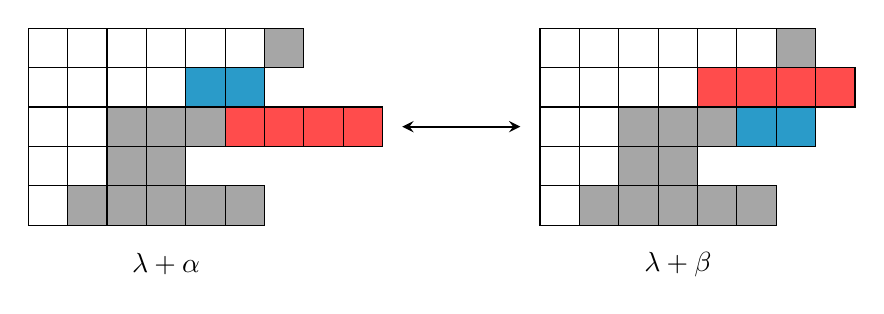
\begin{tikzpicture}[
                x=0.5cm, y=0.5cm,
                square/.style={draw, minimum size=0.5cm},
                white/.style={fill=white},
                gray/.style={fill=gray!70},
                blue/.style={fill=cyan!80!black},
                green/.style={fill=green!80!black},
                red/.style={fill=red!70!white}
            ]
            \begin{scope}[shift={(0,0)}]
                % First Row
                \foreach \x in {0,1,2,3,4,5} { \node[square, white] at (\x,4) {}; }
                \node[square, gray] at (6,4) {};
    
                % Second Row
                \foreach \x in {0,1,2,3} { \node[square, white] at (\x,3) {}; }
                \foreach \x in {4,5} { \node[square, blue] at (\x,3) {}; }
    
                % Third Row
                \foreach \x in {0,1} { \node[square, white] at (\x,2) {}; }
                \foreach \x in {2,3,4} { \node[square, gray] at (\x,2) {}; }
                \foreach \x in {5,6,7,8} { \node[square, red] at (\x,2) {}; }
    
                % Fourth Row
                \foreach \x in {0,1} { \node[square, white] at (\x,1) {}; }
                \foreach \x in {2,3} { \node[square, gray] at (\x,1) {}; }
    
                % Fifth Row
                \node[square, white] at (0,0) {};
                \foreach \x in {1,2,3,4,5} { \node[square, gray] at (\x,0) {}; }
            \end{scope}
            \node at (3, -1.5) {$\lambda + \alpha$};
            \begin{scope}[shift={(13,0)}] % Position of the second grid
                % First Row
                \foreach \x in {0,1,2,3,4,5} { \node[square, white] at (\x,4) {}; }
                \node[square, gray] at (6,4) {};
    
                % Second Row
                \foreach \x in {0,1,2,3} { \node[square, white] at (\x,3) {}; }
                \foreach \x in {4,5,6,7} { \node[square, red] at (\x,3) {}; }
    
                % Third Row
                \foreach \x in {0,1} { \node[square, white] at (\x,2) {}; }
                \foreach \x in {2,3,4} { \node[square, gray] at (\x,2) {}; }
                \foreach \x in {5,6} { \node[square, blue] at (\x,2) {}; }
    
                % Fourth Row
                \foreach \x in {0,1} { \node[square, white] at (\x,1) {}; }
                \foreach \x in {2,3} { \node[square, gray] at (\x,1) {}; }
    
                % Fifth Row
                \node[square, white] at (0,0) {};
                \foreach \x in {1,2,3,4,5} { \node[square, gray] at (\x,0) {}; }
            \end{scope}
            \node at (16, -1.5) {$\lambda + \beta$};
            \draw[<->, thick, >=stealth] (9,2) -- (12,2) node[midway, above] {};
    
        \end{tikzpicture}
        \caption{Example of the involution in the proof of Pieri's \(h\)-formula.}
        \label{fig:pieri-h-formula-involution}
    \end{figure}
    
    This map from \(\mathcal{B}\) to itself is an involution,
    and it satisfies that
        \(\lambda + \alpha + \delta_n\)
        \(\lambda + \beta + \delta_n\)
    differ by one transposition,
    hence
    \begin{equation}
        \tilde{a}_{\lambda + \alpha + \delta_n} + \tilde{a}_{\lambda + \beta + \delta_n} = 0.
    \end{equation}
    Finally,
    this implies that
    \begin{equation}
        \sum_{\alpha \in \mathcal{B}}
        \tilde{a}_{\lambda + \alpha + \delta_n}
        = 0,
    \end{equation}
    and consequently
    \begin{align}
        \tilde{a}_{\lambda + \delta_n} h_k
        &= \sum_{\substack{\text{compositions } \alpha \\ \text{of } k \text{ with length } n \\ (\lambda + \alpha) \setminus \lambda \text{ is a horizontal strip}}}
        \tilde{a}_{\lambda + \alpha + \delta_n} \\
        &= \sum_{\substack{\text{partitions } \mu \\ \lambda \setminus \mu \text{ is a Horizontal strip of size } k}}
        \tilde{a}_{\mu + \delta_n}.
    \end{align}
    Therefore,
    \begin{equation}
        a_\lambda h_k = \sum_{\mu} a_{\mu},
    \end{equation}
    where the sum is over all partitions \(\mu\) obtained by adding a horizontal strip of size \(k\) to \(\lambda\).
    Finally, the result follows by dividing by \(v_n\).
\end{proof}

In the next section, we solve a problem that we didn't even know we wanted to solve:
\emph{How to write \(h_\lambda\) and \(e_\lambda\) in the Schur basis?}

\section{Tableaux and Kostka Numbers}

\begin{definition}[Semistandard Young tableaux]
    A \vocab{semistandard tableaux \(T\)} 
    is a sequence of nested partitions
    \begin{equation}
        \varnothing = \lambda^{(0)}
        \subset \lambda^{(1)}
        \subset \cdots
        \subset \lambda^{(\ell)},
    \end{equation}
    such that \(\lambda^{(k)} \setminus \lambda^{(k-1)}\) is a horizontal strip, for all \(k \in \interval{\ell}\).
    We say that \(T\) has \vocab{shape} \(\lambda = \lambda^{(\ell)}\).
\end{definition}

Traditionally, a semistandard tableau \(T\) of shape \(\lambda\) is represented by filling the boxes of the diagram of \(\lambda\) with numbers from the set \(\{1, 2, \ldots, \ell\}\). Specifically, the number \(i\) is placed in the boxes corresponding to the horizontal strip \(\lambda^{(i)} \setminus \lambda^{(i-1)}\).

Under this depiction, a filling of the boxes of a Young diagram is semistandard if and only if the entries in each row are weakly increasing from left to right, and the entries in each column are strictly increasing from top to bottom.

\begin{example}
    Consider the following semistandard tableaux of shape \(\composition{5, 4, 2}\):
    \begin{equation}
        \varnothing
        \subset \composition{3}
        \subset \composition{4, 2}
        \subset \composition{4, 2}
        \subset \composition{5, 4}
        \subset \composition{5, 4, 2}.
    \end{equation}
    This tableaux is drawn as
    \begin{equation}
        \begin{ytableau}
            1 & 1 & 1 & 2 & 4 \\
            2 & 2 & 4 & 4 \\
            5 & 5
        \end{ytableau}.
    \end{equation}
\end{example}

The \vocab{weight} (sometimes called \vocab{content}) of a tableaux
is the composition \(\alpha\) such that the number \(i\) appears \(\alpha_i\) times in the tableaux, that is, \(\alpha_i\) is the size of the horizontal strip \(\lambda^{(i)} \setminus \lambda^{(i-1)}\).

\begin{definition}[Standard Young tableaux]
    A \vocab{standard tableaux} is a semistandard Young tableaux with weight \(\composition{1, 1, \ldots, 1}\), that is, each horizontal strip has size \(1\).
\end{definition}

\begin{definition}[Kostka numbers]
    Let \(\lambda\) be a partition and \(\alpha\) be a composition.
    The \vocab{Kostka number} \(K_{\lambda \alpha}\) is the number of standard Young tableaux of shape \(\lambda\) and weight \(\alpha\).
\end{definition}

\begin{theorem} \label{thm:h-e-sum-kostka-schur}
    Let \(\alpha\) be a composition.
    Then,
    \begin{equation}
        h_\alpha = \sum_{\lambda} K_{\lambda \alpha} s_\lambda,
    \end{equation}
    and
    \begin{equation}
        e_\alpha = \sum_{\lambda} K_{\lambda \alpha} s_{\tilde\lambda}.
    \end{equation}
\end{theorem}

\begin{proof}
    Note that 
    \begin{align}
        h_\alpha
        &= h_{\alpha_1} h_{\alpha_2} \cdots h_{\alpha_\ell} \\
        &= s_{\varnothing} h_{\alpha_1} s_{\varnothing} h_{\alpha_2} \cdots s_{\varnothing} h_{\alpha_\ell},
    \end{align}
    and then the result follows by successively applying \nameref{thm:pieri-h-formula}.
    The proof for the \(e\)-formula is similar, using \nameref{thm:pieri-e-formula}.
\end{proof}

We list some observations about Kostka numbers.

\begin{corollary} \label{cor:kostka-composition-sort}
    Let \(\alpha\) be a composition and let \(\mu = \overline{\alpha}\).
    Then, \(K_{\lambda \alpha} = K_{\lambda \mu}\).
\end{corollary}

\begin{proof}
    Since \(h_\alpha = h_\mu\), the result follows from Theorem~\ref{thm:h-e-sum-kostka-schur} and the fact that the Schur polynomials are linearly independent.
\end{proof}

\begin{fact}
    If \(|\lambda| \neq |\mu|\), then \(K_{\lambda \mu} = 0\).
\end{fact}

\begin{fact}
    Let \(\lambda\) be a partition.
    Then \(K_{\lambda \lambda} = 1\).
\end{fact}

The only standard Young tableaux of shape \(\lambda\) and weight \(\lambda\) is the one where the number \(i\) is placed in the \(i\)\textsuperscript{th} box of the \(i\)\textsuperscript{th} row.
This tableaux is called \vocab{Yamanouchi tableaux}, \vocab{the highest weight tableaux of shape \(\lambda\)}, or \vocab{supersemistandard tableaux}.

\begin{fact}
    Let \(\lambda, \mu\) be partitions.
    If \(K_{\lambda \mu} \neq 0\), then \(\lambda \geq \mu\).
\end{fact}

\begin{proof}
    Let \(i\) be a positive integer.
    The entries of a standard Young tableaux of shape \(\lambda\) and weight \(\mu\) that are at most \(i\) must be contained in the first \(i\) rows of the Young diagram of \(\lambda\).
    Therefore, \(\lambda_1 + \cdots + \lambda_i \geq \mu_1 + \cdots + \mu_i\) for all \(i\),
    and consequently, \(\lambda \geq \mu\).
\end{proof}

\begin{fact}
    Kostka numbers are not symmetric, that is, 
    there exist partitions \(\lambda, \mu\) such that \(K_{\lambda \mu} \neq K_{\mu \lambda}\).
\end{fact}

\begin{example}
    Let \(\lambda = \composition{2}\) and \(\mu = \composition{1, 1}\).
    Then, \(K_{\lambda \mu} = 1\) and \(K_{\mu \lambda} = 0\).
\end{example}

The \vocab{Kostka matrix} \(K\) is the matrix where the entry in the \(\mu\)\textsuperscript{th} row and \(\lambda\)\textsuperscript{th} column is \(K_{\lambda \mu}\) (note the reversal of indices).
Note that \(K\) is upper triangular (with respect a linear extension of the dominance order) and its diagonal entries are all \(1\).
Therefore, \(K\) is invertible, and its inverse has integer entries.
We call \(K^{-1}\) the \vocab{inverse Kostka matrix}.
Let \(K^{-1}_{\lambda \mu}\) be the entry in the \(\mu\)\textsuperscript{th} row and \(\lambda\)\textsuperscript{th} column of \(K^{-1}\).

\begin{theorem}
    Let \(\lambda\) be a partition.
    Then,
    \begin{equation}
        \omega(s_\lambda) = s_{\tilde\lambda}.
    \end{equation}
\end{theorem}

\begin{proof}
    Theorem~\ref{thm:h-e-sum-kostka-schur} implies that
    \begin{equation}
        s_\lambda = \sum_{\mu} K_{\lambda \mu}^{-1} h_\mu,
    \end{equation}
    and 
    \begin{equation}
        s_{\tilde\lambda} = \sum_{\mu} K_{\lambda \mu}^{-1} e_\mu.
    \end{equation}
    It is straightforward to check that applying \(\omega\) to the right-hand side of the first equation gives the right-hand side of the second equation, and the result follows.
\end{proof}

\begin{theorem}[Jacobi--Trudi's determinant formula] \label{thm:jacobi-trudi}
    Let \(\lambda\) be a partition and let \(n \geq \ell(\lambda)\) be an integer.
    Then,
    \begin{equation}
        s_\lambda = \det\left( s_{\lambda_i + n - i - j} \right)_{i, j \in \interval{n}}.
    \end{equation}
    and
    \begin{equation}
        s_{\tilde\lambda} = \det\left( s_{\lambda_i + n - i - j} \right)_{i, j \in \interval{n}}.
    \end{equation}
\end{theorem}

\begin{example}
    Let's compute \(s_{\composition{3, 1}}\) using \nameref{thm:jacobi-trudi}.
    Let \(n = 4\).
    We have
    \begin{equation}
        s_{\composition{3, 1}}
        = \left|
            \begin{matrix}
                h_3 & h_4 & h_5 & h_6 \\
                h_0 & h_1 & h_2 & h_3 \\
                0   & 0   & h_0 & h_1 \\
                0   & 0   & 0   & h_0
            \end{matrix}
        \right|
        = \left|
            \begin{matrix}
                h_3 & h_4 \\
                h_0 & h_1 \\
            \end{matrix}
        \right|
        = h_{\composition{3, 1}} - h_{\composition{4}},
    \end{equation}
    and
    \begin{equation}
        s_{\composition{3, 1}} = s_{\tilde{\composition{2, 1, 1}}} =
        \left|
            \begin{matrix}
                e_2 & e_3 & e_4 \\
                e_0 & e_1 & e_2 \\
                0   & e_0 & e_1
            \end{matrix}
        \right|
        = e_{\composition{2, 1, 1}} + e_{\composition{4}} - e_{\composition{3, 1}} - e_{\composition{2, 2}}.
    \end{equation}
\end{example}

\begin{proof}[Proof of \nameref{thm:jacobi-trudi}]
    It is straightforward to check that the determinants are equal for all \(n \geq \ell(\lambda)\). Therefore, it suffices to prove the result for \(n = \ell(\lambda)\).

    We proceed by induciton on \(n = \ell(\lambda)\).
    The result is true for \(n = 0\).

    We column expand along the rightmost column
    \begin{equation}
        \det\left( s_{\lambda_i + \ell - i - j} \right)_{i, j \in \interval{n}}
        =
        \sum_{i=1}^\ell
        (-1)^{\ell - i}
        h_{\lambda_i + \ell - i}
        s_{\composition{\lambda_1, \ldots, \lambda_{i-1}, \lambda_{i+1} - 1, \ldots, \lambda_\ell - 1}}
    \end{equation}

    \textcolor{red}{... I did not finish this proof. Reading a book proof might be better.}
\end{proof}

\begin{theorem}
    \begin{equation}
        \prod_{i, j} (1 - x_i y_j)^{-1} = \sum_{\lambda} s_\lambda(x) s_{\lambda}(y).
    \end{equation}
\end{theorem}

\begin{proof}
    By \nameref{thm:jacobi-trudi}, we have
    \begin{equation}
        s_\lambda = \sum_{w \in \sym_n} \sign(w) h_{\lambda + \delta - w \cdot \delta}.
    \end{equation}
    Multiplying by \(v_n\) gives
    \begin{equation}
        a_\lambda = a_\varnothing \sum_{w \in \sym_n} \sign(w) h_{\lambda + \delta - w \cdot \delta}.
    \end{equation}
    Let \(\alpha = \lambda + \delta\).
    Then,
    \begin{equation}
        \tilde{a}_\alpha = \tilde{a}_\delta \sum_{w \in \sym_n} \sign(w) h_{\alpha - w \cdot \delta}.
    \end{equation}

    Now, recall that
    \begin{equation}
        \prod_{i, j} (1 - x_i y_j)^{-1} = \sum_{\lambda} h_\lambda(x) m_\lambda(y) = \sum_{\gamma} h_{\overleftarrow{\gamma}}(x) x^\gamma,
    \end{equation}
    and consequently
    \begin{align}
        \tilde{a}_\delta(x) \tilde{a}_\delta(y) 
        \prod_{i, j} (1 - x_i y_j)^{-1}
        &= \tilde{a}_\delta(x) \sum_{\gamma} \sum_{w \in \sym_n} \sign(w) h_{\overleftarrow{\gamma}}(x) y^{\gamma} \\
        &= \textcolor{red}{... TBD}.
    \end{align}
\end{proof}

\begin{corollary}
    Let \(\lambda, \mu\) be partitions.
    Then,
    \begin{equation}
        \langle s_\lambda, s_\mu \rangle = \delta_{\lambda \mu}.
    \end{equation}
\end{corollary}

\begin{corollary} \label{cor:schur-sum-kostka-m}
    Let \(\lambda\) be a partition.
    Then,
    \begin{equation}
        s_\lambda = \sum_{\mu} K_{\lambda \mu} m_\mu.
    \end{equation}
\end{corollary}

\begin{proof}
    Define \(Q_{\lambda, \xi}\) so that \(s_\lambda = \sum_{\xi} Q_{\lambda, \xi} m_\xi\).
    On the one hand, we have
    \begin{equation}
        \langle h_\mu, s_\lambda \rangle
        = \langle h_\mu, \sum_{\xi} Q_{\lambda, \xi} m_\xi \rangle
        = \sum_{\xi} Q_{\lambda, \xi} \langle h_\mu, m_\xi \rangle
        = Q_{\lambda, \mu}.
    \end{equation}
    On the other hand, we have
    \begin{equation}
        \langle h_\mu, s_\lambda \rangle
        = \langle \sum_{\nu} K_{\nu \mu} s_\nu, s_\lambda \rangle
        = \sum_{\nu} K_{\nu \mu} \langle s_\nu, s_\lambda \rangle
        = K_{\lambda \mu}.
    \end{equation}
    Therefore, \(Q_{\lambda, \mu} = K_{\lambda \mu}\), and the result follows.
\end{proof}

\begin{example}[\(s_{\composition{2, 1}}\)]
    Let's compute \(s_{\composition{2, 1}}\) using Corollary~\ref{cor:schur-sum-kostka-m}.
    We have
    \begin{equation}
        s_{\composition{2, 1}}
        =
        0 m_{\composition{3}} + 
        1 m_{\composition{2, 1}} +
        2 m_{\composition{1, 1, 1}}.
    \end{equation}
\end{example}

\begin{example}[\(s_{\composition{4, 2}}\)]
    Let's compute \(s_{\composition{4, 2}}\) using Corollary~\ref{cor:schur-sum-kostka-m}.
    We have
    \begin{equation}
        s_{\composition{4, 2}}
        =
        1 m_{\composition{4, 2}} +
        1 m_{\composition{4, 1, 1}} +
        1 m_{\composition{3, 3}} +
        2 m_{\composition{3, 2, 1}} +
        3 m_{\composition{3, 1, 1, 1}} +
        3 m_{\composition{2, 2, 2}} +
        6 m_{\composition{2, 2, 1, 1}} +
        4 m_{\composition{2, 1, 1, 1, 1}} +
        9 m_{\composition{1, 1, 1, 1, 1, 1}}.
    \end{equation}
\end{example}

From Corollary~\ref{cor:schur-sum-kostka-m}, we can observe that, for all nonnegative integers \(k\),
\begin{equation}
    s_{\composition{1}^k} = e_k
    \qquad \text{and} \qquad
    s_{\composition{k}} = h_k.
\end{equation}

\begin{corollary}
    Let \(\lambda\) be a partition.
    Then,
    \begin{equation}
        s_{\lambda} = \sum_{\text{semistandard tableaux } T \text{ of shape } \lambda} x^{\wt(T)},
    \end{equation}
    where \(\wt(T)\) is the weight of \(T\).
\end{corollary}

\begin{proof}
    By Corollary~\ref{cor:schur-sum-kostka-m}, we have
    \begin{equation}
        s_{\lambda} = \sum_{\mu} K_{\lambda \mu} m_{\mu}
        = \sum_{\alpha} K_{\lambda \alpha} x^{\alpha}
        = \sum_{\text{semistandard tableaux } T \text{ of shape } \lambda} x^{\wt(T)}. \qedhere
    \end{equation}
\end{proof}

We provide a combinatorial proof of Corollary~\ref{cor:kostka-composition-sort}, restated below.
\begin{fact}
    Let \(\alpha\) and \(\beta\) be compositions such that \(\overline{\alpha} = \overline{\beta} = \mu\).  Then, \(K_{\lambda \alpha} = K_{\lambda \beta}\).
\end{fact}
\begin{proof}[Proof by Bender--Knuth, 1972]
    By induction, it suffices to show that the result is true when \(\alpha\) and \(\beta\) differ by swapping coordinates \(i\) and \(i+1\).
    Define the \vocab{\(i\)\textsubscript{th} Bender--Knuth involution}
    \begin{equation}
        \operatorname{BK}_i \colon SSYT(\mu) \to SSYT(\mu)
    \end{equation}
    as follows.
    If entries \(i\) and \(i+1\) are in the column, we say that these labels are \emph{frozen}.
    The remaining entries \(i\) and \(i+1\) are said to be \emph{free}.
    It is straightforward to check that, in each row, the free entries look like
    \begin{equation}
        \ytableausetup{boxsize=1cm}
        \begin{ytableau}
            i & i & \cdots & i & i+1 & i+1 & \cdots & i+1
        \end{ytableau}.
    \end{equation}
    Suppose row \(k\) has \(a\) free entries \(i\) and \(b\) free entries \(i+1\).
    The involution \(\operatorname{BK}_i\) swaps those entires to \(b\) entries \(i\) and \(a\) entries \(i+1\).
    In other words, the middle \(|a-b|\) free entries are swapped.
    By doing this to all rows, we obtain a bijection between the set of semistandard tableaux of shape \(\lambda\) and weight \(\alpha\) and the set of semistandard tableaux of shape \(\lambda\) and weight \(\beta\), and the result follows.
\end{proof}

\begin{remark}
    The Bender--Knuth involutions do not satisfy braid relations,
    and therefore they do not generate the symmetric group.
    Instead, we get elements that satisfy
    \begin{gather}
        \operatorname{BK}_i^2 = \operatorname{id}, \\
        \operatorname{BK}_i \operatorname{BK}_j = \operatorname{BK}_j \operatorname{BK}_i \quad \text{if } |i - j| > 1, \\
        (\operatorname{BK}_1 \operatorname{BK}_2)^6 = \operatorname{id},
    \end{gather}
    and, by letting \(q_i =
    \operatorname{BK}_1
    (\operatorname{BK}_2 \operatorname{BK}_1)
    (\operatorname{BK}_3 \operatorname{BK}_2 \operatorname{BK}_1)
    \cdots
    (\operatorname{BK}_i \cdots \operatorname{BK}_2 \operatorname{BK}_1)\),
    we get that, for \(i \geq 2\),
    \begin{equation}
        (\operatorname{BK}_i q_i)^4 = \operatorname{id}.
    \end{equation}
    There are more relations, but nobody knows the entire list.
\end{remark}

    \printbibliography
\end{document}
